\documentclass[10pt,twocolumn,letterpaper]{article}

\usepackage[T1]{fontenc}
\usepackage[utf8]{inputenc}
\usepackage{lmodern}
\usepackage[letterpaper,margin=0.6in,columnsep=0.25in]{geometry}
\usepackage{amsmath,amssymb}
\usepackage{graphicx}
\usepackage{booktabs,tabularx,array}
\usepackage[font=footnotesize,labelfont=bf,labelsep=period,justification=justified,singlelinecheck=false]{caption}
\usepackage{braket}
\usepackage{xcolor}
\usepackage{titlesec}
\usepackage[numbers,sort&compress]{natbib}
\usepackage{microtype}
\usepackage[colorlinks=true,linkcolor=blue!45!black,citecolor=blue!45!black,urlcolor=blue!45!black]{hyperref}

\titleformat{\section}{\normalfont\large\bfseries}{\thesection}{0.6em}{}
\titleformat{\subsection}{\normalfont\normalsize\bfseries}{\thesubsection}{0.5em}{}
\titlespacing*{\section}{0pt}{1.6ex plus 0.5ex minus 0.3ex}{0.7ex plus 0.2ex}
\titlespacing*{\subsection}{0pt}{1.1ex plus 0.3ex minus 0.2ex}{0.4ex plus 0.1ex}
\setlength{\bibsep}{0.6pt}
\renewcommand{\bibfont}{\footnotesize\raggedright}
\setlength{\textfloatsep}{9pt plus 2pt minus 3pt}
\setlength{\dbltextfloatsep}{9pt plus 2pt minus 3pt}
\setlength{\floatsep}{8pt plus 2pt minus 2pt}
\setlength{\dblfloatsep}{8pt plus 2pt minus 2pt}
\setlength{\abovecaptionskip}{3pt}
\renewcommand{\topfraction}{0.9}
\renewcommand{\dbltopfraction}{0.9}
\renewcommand{\bottomfraction}{0.6}
\renewcommand{\textfraction}{0.07}
\renewcommand{\floatpagefraction}{0.85}
\renewcommand{\dblfloatpagefraction}{0.85}
\setcounter{topnumber}{3}
\setcounter{dbltopnumber}{3}
\setcounter{totalnumber}{5}
\raggedbottom

\newcommand{\ee}[1]{\ensuremath{\times10^{#1}}}
\newcommand{\kt}{\tilde{k}}
\newcommand{\ud}{\mathrm{d}}
\newcommand{\doi}[1]{\href{https://doi.org/#1}{\nolinkurl{doi:#1}}}
\newcommand{\arxiv}[1]{\href{https://arxiv.org/abs/#1}{\nolinkurl{arXiv:#1}}}
\newcommand{\file}[1]{\texttt{#1}}

\hypersetup{pdftitle={A collision-driven entangling gate between two flying quantum fluxons with a velocity sweet spot: a simulation study},
            pdfauthor={QBF-X2 project (EE143 Silicon Qubits)}}

\begin{document}

\twocolumn[{%
\begin{center}
{\LARGE\bfseries A collision-driven entangling gate between two flying quantum fluxons with a velocity sweet spot:
a simulation study\par}
\vspace{0.6em}
{\large QBF-X2 project (EE143 Silicon Qubits)\par}
\vspace{0.25em}
{\small November 2026\par}
\end{center}
\vspace{0.1em}
\begin{quote}
\small
\textbf{Abstract.}
We propose QBF-X2, a superconducting circuit in which two quantum fluxons travel in opposite directions on coupled
Josephson transmission lines and leave entangled. We study it by simulation only, and nothing has been built or
measured. Each fluxon is a dual-rail flying qubit, and only the rail-1 lines of the two qubits are coupled, so only the
$\ket{11}$ branch acquires the collision phase $\Delta$, and $\Delta=\pi$ gives a controlled-Z (CZ) gate. An inductive coupler
gives $\Delta\propto1/v$ and a conditional time shift that records the branch. A capacitive coupler, whose phase grows
$\propto v$ for counter-propagating fluxons, makes $\Delta(v)=a/v+bv$ stationary at $v^*=(a/b)^{1/2}$, where the
conditional time shift vanishes and a spread of launch speeds enters only at second order. Exact two-dimensional
scattering of a collective-coordinate Hamiltonian derived from the circuit, with the coupler calibrated at
$\beta^*=v^*/c_0=0.30$, gives $\Delta$ within $1.7\ee{-3}$~rad of $\pi$, a concurrence of 0.9999995 from
$\ket{+}\ket{+}$ and a CZ process fidelity of 0.999999. For a thermal launch at 20~mK the gate error is $1.2\ee{-5}$ at
the sweet spot and $3.8\ee{-3}$ with an inductive-only coupler. The device-feasibility milestone is not met: at the
optimised speed $\beta=0.45$ the realistic error budget for a 300-cell flight is 1.9\%, of which 1.8\% is dephasing
caused by 2\% junction disorder, and the coherent single-fluxon launcher and the layout are unverified.
\end{quote}
\vspace{0.6em}
}]

\section{Introduction}
\label{sec:intro}

A flying qubit carries quantum information between distant parts of a processor. Superconducting circuits use
travelling microwave photons for this, with remote entanglement and state transfer at fidelities of about 73--80\%
\cite{Kurpiers2018,Axline2018,CampagneIbarcq2018}. Dual-rail flying electrons coupled by the Coulomb interaction were
proposed as an in-flight two-qubit gate \cite{Bertoni2000,Ionicioiu2001}, and Coulomb collisions of single flying
electrons have been resolved, so far without an entangling gate \cite{Fletcher2023,Ubbelohde2023,Wang2023}.

A fluxon, or Josephson vortex, is a $2\pi$ kink of the superconducting phase that carries one flux quantum $\Phi_0$.
In a long Josephson junction (LJJ) or a junction array it is a sine-Gordon soliton that moves ballistically and keeps
its identity in collisions \cite{Ustinov1998}. Classical reversible fluxon logic encodes a bit in the polarity of a
fluxon and uses the interaction of two synchronised fluxons to switch the output line of one of them, keeping more than
97\% of the energy \cite{WustmannOsborn2020,Osborn2017}. Fluxons can also be quantum particles: quantised levels and
tunnelling of a vortex were measured in an LJJ \cite{Wallraff2003}, coherent tunnelling between the cells of
high-impedance arrays was predicted \cite{SeidovFistul2021} and reported \cite{Wildermuth2023}, and pinned vortices in
granular aluminium were operated as qubits \cite{Nambisan2026}. In the sources we searched (Sec.~\ref{sec:prior}) we
found no gate in which two flying quantum fluxons are entangled by a coherent collision.

This paper proposes and simulates such a gate, QBF-X2. Each qubit is dual-rail: $\ket{0}$ is a fluxon in rail 0 and
$\ket{1}$ a fluxon in rail 1. Only the rail-1 lines of qubits A and B are coupled, so only the $\ket{11}$ branch
acquires the collision phase $\Delta$, and $\Delta=\pi$ is a CZ gate. The rails are high-impedance junction arrays in
which the fluxon rest energy is only 15.8 plasma quanta (quantum sine-Gordon coupling $\beta^2=0.51$), so the fluxon is
a quantum particle with a de Broglie wavelength of about three cells. A heavy classical fluxon, such as the kick-line
fluxon of the earlier QFX-1 design in the same repository (rest energy 213~THz$\cdot h$), cannot carry a dual-rail
qubit or become entangled in this way.

From the circuit Lagrangian we derive a first-order collective-coordinate Hamiltonian for two light fluxons on
coupled rails and test it against the circuit (Secs.~\ref{sec:circuit} and~\ref{sec:quantum}). Combined inductive and
capacitive coupling makes $\Delta$ stationary in speed, which we call the velocity sweet spot (Sec.~\ref{sec:sweet}).
Exact two-dimensional (2D) scattering then gives a CZ gate with process fidelity 0.999999 for pure wavepackets
(Sec.~\ref{sec:results}), and an error budget shows that junction disorder, not the collision, limits the device to a
1.9\% error at $\beta=0.45$ (Sec.~\ref{sec:budget}). We also give a preliminary netlist, layout and measurement plan
(Sec.~\ref{sec:device}) and five companion devices, one of them a negative result (Sec.~\ref{sec:companions}). Four
milestones with explicit checks organise the work, A (classical ballistic physics), B (quantum ballistic physics),
C (a genuine quantum gate) and D (device feasibility); A, B and C pass, and D is not met
(Appendix~\ref{app:milestones}). All results are simulations.

\section{Prior work}
\label{sec:prior}

\emph{Classical fluxon gates and collisions.} Wustmann and Osborn obtained ballistic one-bit gates from resonant
fluxon scattering at junction interfaces and a two-bit gate from two synchronised fluxons that interact at a shared
interface \cite{WustmannOsborn2020}. A patent \cite{Osborn2017} and related patents \cite{RelatedPatents} use a
fluxon--fluxon interaction to steer a target fluxon into one of two output lines. The same authors proposed qubit
readout through the transmission of a single fluxon, which serves only as a probe \cite{WustmannOsborn2026}. Coupled
sine-Gordon equations are the standard model of stacked junctions \cite{Sakai1993}, in which coherent vortex motion was
studied \cite{Kleiner1994}. Collisions of fluxons
in different coupled junctions \cite{KivsharMalomed1988}, velocity-dependent bunching with inductive and capacitive
coupling \cite{GronbechJensen1994} and the measured repulsion at low and attraction at high velocity between fluxons in
neighbouring layers \cite{UstinovKohlstedt1996} are classical results; measured fluxon--antifluxon collisions gave
negative phase shifts that the authors attribute to dissipation \cite{Fujimaki1987,Nakajima1990}.

\emph{Quantum solitons and vortices.} The exact quantum sine-Gordon S-matrix contains two-body phases that depend on
the rapidity difference \cite{Zamolodchikov1979}, the origin of both a collision phase and its Wigner delay.
Superconducting circuits were proposed as simulators of this scattering \cite{RoySaleur2019,Roy2021,Rosen2026}, not as
gates. For Ref.~\cite{Wildermuth2023} we rely on its abstract (see also \cite{Wildermuth2022}). Aharonov--Casher
interference of vortices \cite{Elion1993}, quantum vortices in one-dimensional arrays \cite{vanOudenaarden1996},
Aharonov--Casher interference of quantum phase slips \cite{Pop2012} and fluxon quantum beats between two cells
\cite{Moskalenko2021} establish the elementary process of our beam splitter. Classical ballistic vortices were observed
in a two-dimensional array \cite{vanderZant1992}.

\emph{Mobile qubits and mediated gates.} Fujii \emph{et al.} proposed flying superconducting qubits made of an
elementary excitation of circuits with Josephson transmission lines \cite{Fujii2007} (we have read only the abstract)
and a quantum breather as a mobile qubit \cite{Fujii2008}; a moving classical fluxon gates stationary qubits in
Refs.~\cite{Matsuo2007,Fujii2009,Fujii2016}. Deng and Averin describe nSQUID arrays as an effective dual-rail conveyor
whose qubit is carried by a classical fluxon \cite{DengAverin2014}. Fistul and Ustinov proposed a cavity-mediated
coupling proportional to the product of the fluxon velocities for trapped vortex qubits \cite{FistulUstinov2003}, and
a patent couples static LJJ vortex qubits magnetically \cite{DWavePatent}. On other platforms, collision CZ gates
between counter-propagating particles have been derived \cite{BoseKorepin2011,Banchi2017}, and distributed cross-Kerr
sites suppress spectral entanglement in photon collisions \cite{BrodCombes2016}.

\emph{What QBF-X2 adds.} The prior-art search of this project (literature databases and web and patent search,
November 2026) rated four elements. The quantum two-fluxon collision gate, which produces a phase on superpositions
instead of switching an output line, and the dual-rail flying-fluxon encoding are partially anticipated. A beam
splitter between ladder rows rests on established phase-slip and Aharonov--Casher physics, but the device was not
found. The velocity-sweet-spot coupler, and an architecture that combines all four elements, were not found in the
sources we searched. This
describes the searched sources and is not a proof of novelty: patent claims could not be read, and the full text of
Ref.~\cite{Fujii2007} remains to be checked.

\section{Circuit model}
\label{sec:circuit}

\subsection{Rails and units}
Each rail is a discrete LJJ: at node $n$ a junction ($E_J$, $C$) connects to ground, and a series inductance $L$
connects to node $n+1$. We use $E_J=40$~GHz ($I_c=80.5$~nA), $E_C=8$~GHz ($C=2.42$~fF) and a Josephson length of
$\Lambda=2.5$ cells, $L_J/L=\Lambda^2$ with $L_J=4.09$~nH, so $L=0.654$~nH per 2~$\mu$m cell. The plasma frequency is
$f_p=(8E_JE_C)^{1/2}=50.6$~GHz, and the continuum rest energy is $E_0=8E_J\Lambda=800$~GHz$\cdot h$ (19.955\,$E_J$ for
the relaxed lattice kink). Unless stated otherwise, lengths are in cells, time in $1/\omega_p$ and energy in $E_J$; the
limiting speed is $c_0=\Lambda$ cells per $1/\omega_p$ (1590~$\mu$m/ns), and $\beta=v/c_0$.

\subsection{Rows, couplers and dummy couplers}
Six rows run in parallel: $D_A$, $A0$, $A1$, $B1$, $B0$, $D_B$ (Figs.~\ref{fig:schematic} and~\ref{fig:layout}).
Qubit A moves in $+x$ on $A0$ ($\ket{0}$) or $A1$ ($\ket{1}$), qubit B in $-x$ on $B0$ or $B1$. The gate coupler joins
$A1$ and $B1$ over a plateau with tapered ends (envelope $0\le g(n)\le1$). It combines a mutual inductance $M=kL$ per
cell, from a shared ground-return strip $L_s=kL$ with the series inductance reduced to $(1-k)L$, and a capacitance
$C_c=cC$ between facing nodes, with the node capacitance reduced by $C_c$, so the self-inductance and capacitance of each
rail are unchanged. Identical dummy couplers join $A0$ to $D_A$ and $B0$ to $D_B$, rows without injectors, so both
rails of a qubit have the same single-particle phase and delay. Before and after the coupler the two rows of a qubit
form a ladder whose middle-rail junctions ($E_{J,M}/E_{C,M}=2$) let the fluxon hop between rows by a quantum phase slip
of amplitude $E_S$; a gate voltage sets the Aharonov--Casher phase $\chi$ between the paths (Sec.~\ref{sec:companions}).
Fluxons are launched by a junction with twice the rail critical current, a current pulse and a 40-cell accelerator, and
detected by a catcher loop (20~nH) with dispersive $\lambda/4$ readout, as in QFX-1. The launcher is unresolved.

\begin{figure*}[t]
\centering
\begin{minipage}[c]{0.60\textwidth}\centering
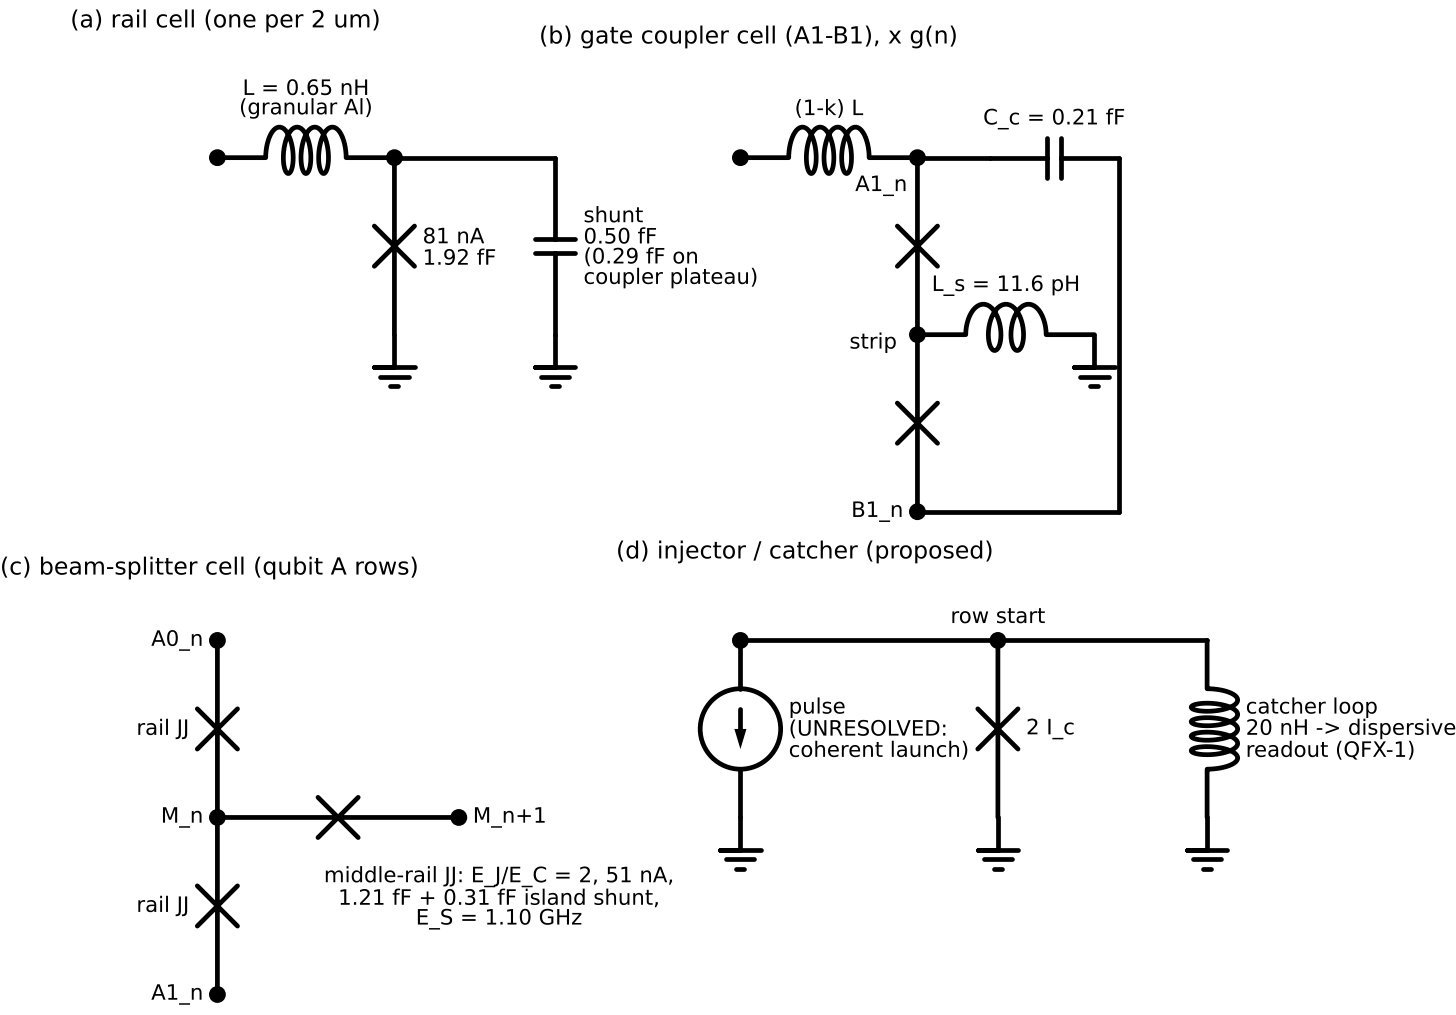
\includegraphics[width=\textwidth]{../circuits/schematic_unit_cells.png}
\end{minipage}\hfill
\begin{minipage}[c]{0.37\textwidth}\centering
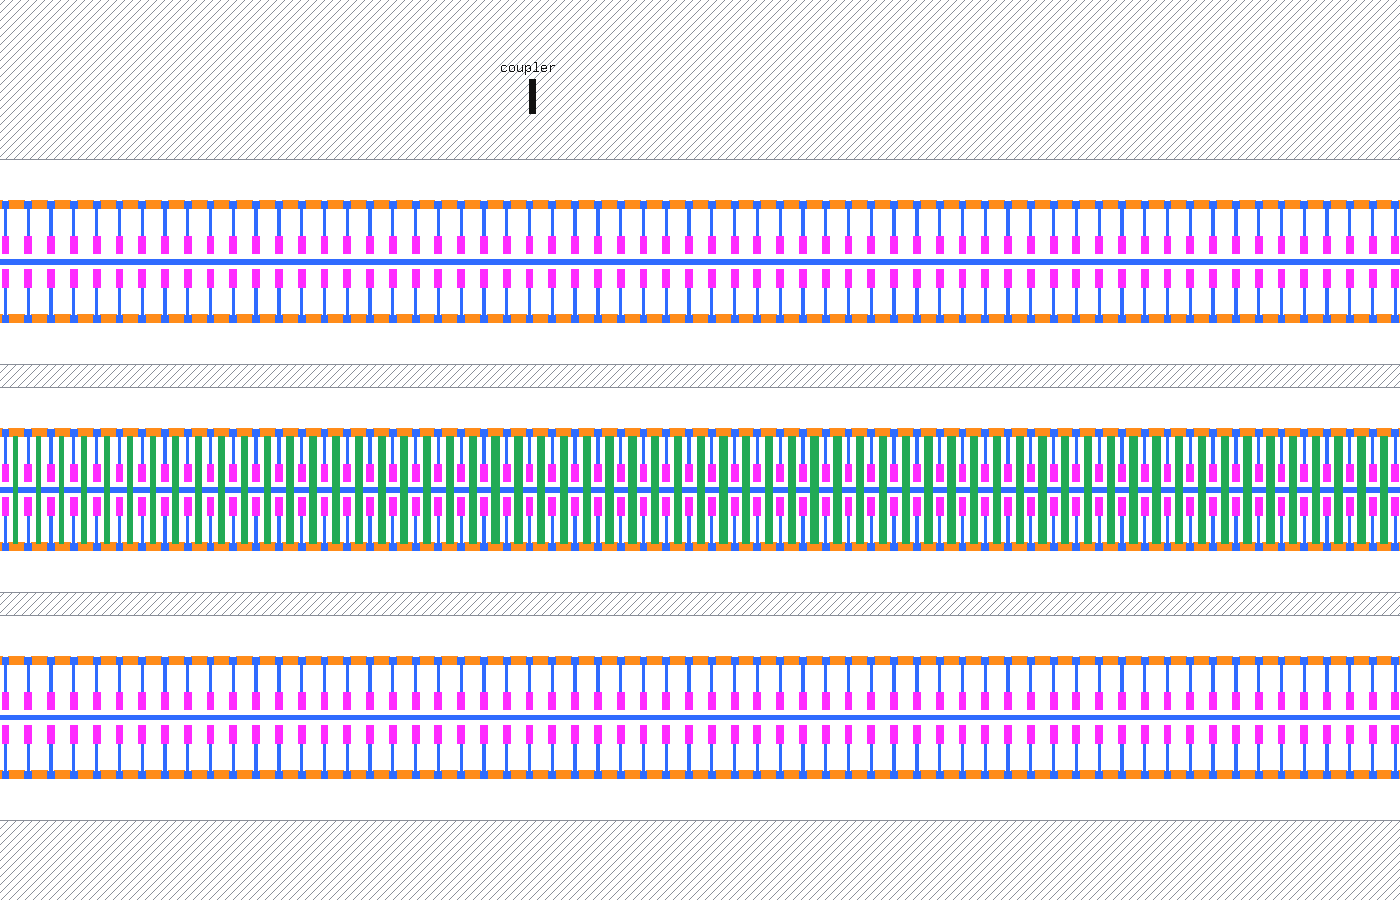
\includegraphics[width=\textwidth]{../circuits/layout_zoom_coupler.png}\\[1pt]
{\footnotesize (e)}
\end{minipage}
\caption{Preliminary QBF-X2 unit cells with the element values of the optimised operating point $\beta=0.45$; none
of this has been fabricated. (a)~Rail cell, one per 2~$\mu$m: $L=0.65$~nH (granular Al), a junction (81~nA, 1.92~fF)
and a node shunt of 0.50~fF (0.29~fF on the coupler plateau) to ground. (b)~Gate-coupler cell between $A1$ and $B1$, scaled by $g(n)$: the ground returns of the two rail
junctions share a strip $L_s=11.6$~pH, which produces the mutual inductance, the series inductance is reduced to
$(1-k)L$, and $C_c=0.21$~fF joins the facing nodes; the dummy couplers are identical. (c)~Beam-splitter cell of
qubit~A: a middle-rail junction with $E_J/E_C=2$ (51~nA, 1.21~fF plus a 0.31~fF island shunt, $E_S=1.10$~GHz).
(d)~Proposed injector (current pulse into a
$2I_c$ junction; coherent launch unresolved) and catcher loop. (e)~Layout zoom in the coupler section: dummy coupler
$D_A$--$A0$ (top), gate coupler $A1$--$B1$ (middle) and dummy coupler $B0$--$D_B$ (bottom), each with coupling-capacitor
crossovers (green); the node and island shunts are not drawn.}
\label{fig:schematic}
\end{figure*}

\subsection{Lagrangian and equations of motion}
With $\boldsymbol\phi_n$ the node phases of all rails at node $n$ and $\mathbf a_n=\boldsymbol\phi_{n+1}-
\boldsymbol\phi_n$ the phase drops across the cell inductors, the circuit Lagrangian is
\begin{equation}
\mathcal L=\sum_n\Big[\tfrac12\dot{\boldsymbol\phi}_n^{\mathsf T}\tilde M_n\dot{\boldsymbol\phi}_n
-\tfrac{\Lambda^2}{2}\mathbf a_n^{\mathsf T}\tilde K_n\mathbf a_n-\sum_r\big(1-\cos\phi_{r,n}\big)\Big],
\label{eq:lagrangian}
\end{equation}
where $\tilde M_n$ is the node capacitance matrix divided by $C$ and $\tilde K_n$ is $L$ times the inverse of the cell
inductance matrix. A coupler between rails $i$ and $j$ sets $(\tilde M_n)_{ij}=-c\,g_n$ and adds $k\,g_n$ to the
off-diagonal entries of the cell inductance matrix in units of $L$; the diagonal entries stay 1 because of the
compensation. The equations of motion are
\begin{equation}
\tilde M_n\ddot{\boldsymbol\phi}_n=\Lambda^2\big(\tilde K_n\mathbf a_n-\tilde K_{n-1}\mathbf a_{n-1}\big)
-\sin\boldsymbol\phi_n-\alpha_n\dot{\boldsymbol\phi}_n+\boldsymbol\gamma_n ,
\label{eq:eom}
\end{equation}
with sub-gap damping $\alpha_n$, bias $\boldsymbol\gamma_n$ and open ends. A kink moving at $v=\beta\Lambda$ is
\begin{equation}
\phi(n,t)=4\arctan\exp\!\big[\gamma(n-X(t))/\Lambda\big],\quad \gamma=(1-\beta^2)^{-1/2}.
\label{eq:kink}
\end{equation}
Table~\ref{tab:params} lists the design parameters and their status.

\begin{table*}[t]
\centering\footnotesize
\caption{Design parameters and their status (\file{FEASIBILITY.\allowbreak{}md}, Sec.~2, cross-checked against
\file{results/\allowbreak{}A\_\allowbreak{}classical.\allowbreak{}json}, \file{C\_\allowbreak{}gate.\allowbreak{}json} and \file{D\_\allowbreak{}feasibility.\allowbreak{}json}). ``Validated'' means validated
by the simulations of this project, not by measurement.}
\label{tab:params}
\begin{tabularx}{\textwidth}{@{}>{\raggedright\arraybackslash}p{0.20\textwidth}>{\raggedright\arraybackslash}p{0.34\textwidth}>{\raggedright\arraybackslash}X@{}}
\toprule
Quantity & Value & Status\\
\midrule
Rail junction $E_J$, $E_C$ & 40~GHz (80.5~nA), 8~GHz (2.42~fF: 1.92~fF junction + 0.50~fF node shunt) & design; quantum regime validated ($\beta^2=0.51$, Peierls--Nabarro barrier $2.9\ee{-6}$~GHz)\\
Rail inductance per cell & 0.654~nH ($\Lambda=2.5$), 1.31 squares of granular Al & proposed (sheet inductance 0.5~nH/$\square$ assumed)\\
Gate coupler, reference $\beta^*=0.30$ & $k=0.01189$, $c=0.1266$ ($L_s\approx7.8$~pH, $C_c\approx0.31$~fF) & validated by exact 2D calibration: $\Delta=\pi$, $\ud\Delta/\ud\beta=0.002$\\
Gate coupler, optimum $\beta=0.45$ & $k=0.01778$, $c=0.0875$ ($L_s=11.6$~pH, $C_c=0.21$~fF) & validated: 2D calibration ($|\Delta-\pi|=1.3\ee{-4}$~rad, $\ud\Delta/\ud\beta=2.2\ee{-5}$); circuit zero crossing at $\beta=0.454$\\
Dummy couplers on $A0$, $B0$ & identical to the gate coupler & proposed; cancel single-particle phases and delays between rails\\
Beam splitter & $E_{J,M}/E_{C,M}=2$ (25.3/12.7~GHz), $E_S=1.10$~GHz & $E_S$ validated from the exact charge dispersion; vortex hopping is a single-junction estimate (unresolved)\\
Launcher & $2I_c$ injection junction, current pulse, 40-cell accelerator & \textbf{unresolved}: motional-state preparation and timing ($\le10$~ps) not modelled\\
Detector & catcher loop (20~nH), dispersive $\lambda/4$ readout as in QFX-1 & proposed\\
Junction disorder & 2\% assumed; $\le1$\% needed for a sub-1\% gate error & \textbf{open} fabrication requirement\\
Damping $\alpha$ & $2\ee{-6}$ assumed (quasiparticle- and dielectric-limited at 20~mK) & unknown; each emitted plasma quantum counted as which-rail information (upper bound)\\
\bottomrule
\end{tabularx}
\end{table*}

\section{Quantum collective-coordinate model}
\label{sec:quantum}

\subsection{Derivation}
We insert two rigid kinks, $\phi_{A1}(n)=f(n-X_A)$ and $\phi_{B1}(n)=f(n-X_B)$, each with the Lorentz-contracted
profile of Eq.~\eqref{eq:kink}, into Eq.~\eqref{eq:lagrangian} and keep terms to first order in $k$ and $c$. The
single-kink terms give the relativistic free Lagrangian with the lattice rest energy $E_0$. The inductive cross term is
$\Lambda^2\kt\sum_n a_Aa_B$, with $\kt=k/(1-k^2)$ from inverting the inductance matrix, and the capacitive one is
$-c\sum_n\dot\phi_A\dot\phi_B=-c\,\dot X_A\dot X_B\sum_n f'(n-X_A)f'(n-X_B)$. With $a(x)=f(x+1)-f(x)$ the phase drop
across one cell, both sums become the overlap $O(r)=\sum_n a(n-X_A)\,a(n-X_B)$, $r=X_A-X_B$, and
\begin{align}
\mathcal L_{\rm cc}={}&-E_0\sqrt{1-\dot X_A^2/c_0^2}-E_0\sqrt{1-\dot X_B^2/c_0^2}\nonumber\\
&+E_J\big[\Lambda^2\kt-c\,\dot X_A\dot X_B\big]\,O(X_A-X_B)\,g\!\left(\tfrac{X_A+X_B}{2}\right).
\label{eq:Lcc}
\end{align}
The velocities are signed. For counter-propagating fluxons $\dot X_A\dot X_B<0$, so the capacitive term has the sign
of the inductive one. Because the phase drops of each kink add up to $2\pi$,
\begin{equation}
\int O(r)\,\ud r=(2\pi)^2 ,
\label{eq:sumrule}
\end{equation}
independent of the kink shape. Canonical quantisation of $X_A$ and $X_B$, with momenta $\hbar k_A$ and $\hbar k_B$,
gives
\begin{align}
H={}&E(k_A)+E(k_B)-E_J\Lambda^2\kt\,O\,g+\frac{cE_J}{2}\big\{u_Au_B,\,O\,g\big\},\label{eq:H}\\
E(k)={}&\sqrt{E_0^2+(\hbar c_0k)^2}-E_0 ,\label{eq:disp}
\end{align}
with the velocity operator $u=\partial E/\partial(\hbar k)$ in cells per $1/\omega_p$ and $\hbar c_0=h\times126.5$~GHz
cell. The velocity coupling depends on the momenta and does not commute with $O(X_A-X_B)g$, so it is ordered
symmetrically with the anticommutator, which makes $H$ Hermitian. Equation~\eqref{eq:disp} is the relativistic
dispersion of the lattice kink, tested in Sec.~\ref{sec:resB}. The model omits $O(k^2,c^2)$ image and renormalisation
terms, which are identical in every logical branch because of the dummy couplers, as well as the Peierls--Nabarro
potential, coupling to plasma modes and dissipation. Each omission is checked or bounded below.

\subsection{Regime of validity}
For these rails the quantum sine-Gordon coupling is $\beta^2=8hf_p/E_0=0.506$, far below $8\pi$, where the soliton
description is lost, and the quantum mass renormalisation is about $\beta^2/8\pi=2.0$\%. The rest energy is 15.8
plasma quanta. The Peierls--Nabarro barrier, $2.9\ee{-6}$~GHz, is negligible against the kinetic energy at
$\beta=0.30$, 38.5~GHz. At $\beta=0.30$ the de Broglie wavelength is 3.17 cells, comparable to the fluxon size
$\Lambda=2.5$ cells, and $k_BT$ at 20~mK is 0.417~GHz.

The first-order theory holds only in a window of speeds. For the inductive-only coupler, its classical shift
(Sec.~\ref{sec:sweet}) agrees with the circuit within 3\% for $\beta=0.28$--$0.32$ but deviates by $-10.8$\% at
$\beta=0.20$, $-16.1$\% at 0.35 and $-24.3$\% at 0.40 (Fig.~\ref{fig:classical}c). Below $\beta\approx0.22$ the
interaction is no longer weak compared with the kinetic energy and the first-order shifts are 10--40\% too large; above
$\beta\approx0.35$ (inductive) to 0.45 (mixed) lattice radiation and $O(c^2)$ dragging take the circuit away from the
rigid-kink theory. For $\Lambda\lesssim1.5$ Peierls--Nabarro pinning and Bloch-band motion would appear, and plasmon
emission is treated only classically. Even at the design point the exact phase exceeds the first-order value by
0.130~rad, a second-order effect removed by calibration (Sec.~\ref{sec:calib}).

\section{The velocity sweet spot}
\label{sec:sweet}

\subsection{Conditional phase}
To first order, the $\ket{11}$ branch acquires the action of the interaction term of Eq.~\eqref{eq:Lcc} along the
unperturbed paths $X_A=v_At$ and $X_B=-v_Bt$. With $\ud r/\ud t=v_A+v_B$, a plateau longer than the interaction range
($g=1$) and Eq.~\eqref{eq:sumrule}, the action is
\begin{equation}
\delta S(v_A,v_B)=(2\pi)^2E_J\,\frac{\Lambda^2\kt+c\,v_Av_B}{v_A+v_B}
\label{eq:dS}
\end{equation}
in units of $E_J/\omega_p$, for speeds $v_A,v_B>0$ in cells per $1/\omega_p$, and the conditional phase is
$\Delta=\delta S/\hbar$,
\begin{equation}
\Delta(v_A,v_B)=(2\pi)^2\frac{E_J}{hf_p}\,\frac{\Lambda^2\kt+c\,v_Av_B}{v_A+v_B}.
\label{eq:Delta}
\end{equation}
For equal speeds $v=\beta\Lambda$,
\begin{equation}
\Delta(\beta)=\Gamma\Big(\frac{\kt}{\beta}+c\beta\Big),\qquad \Gamma=2\pi^2\Lambda\frac{E_J}{hf_p},
\label{eq:Deltabeta}
\end{equation}
of the form $a/v+bv$: the inductive term falls and the capacitive term rises with speed. $\Delta$ is stationary at
\begin{equation}
\beta^{*2}=\kt/c ,\qquad v^*=\Lambda\sqrt{\kt/c}.
\label{eq:betastar}
\end{equation}
A coupler with $\Delta(\beta^*)=\pi$ has $c=\pi/(2\Gamma\beta^*)$ and $\kt=c\beta^{*2}$; for $\beta^*=0.30$ this
first-order design is $k=0.01208$, $c=0.1342$.

\subsection{No conditional time shift at \texorpdfstring{$v^*$}{v*}}
Because $\Delta$ depends on the momenta, the $\ket{11}$ wavepackets are shifted in time by the Wigner time
$\tau=\hbar\,\partial\Delta/\partial E$. Classically, the Hamilton--Jacobi relation gives the position shift of
fluxon A after the collision,
\begin{equation}
\Delta X_A=-\frac{\partial\,\delta S/\partial v_A}{m\gamma_A^3},\qquad m=E_0/c_0^2 ,
\label{eq:shift}
\end{equation}
and at $v_A=v_B=v$, $\partial\,\delta S/\partial v_A=(2\pi)^2(cv^2-\Lambda^2\kt)/(2v)^2$, which vanishes at $v^*$. The
conditional time shift therefore vanishes at the stationary point, classically and quantum mechanically, and the
outgoing $\ket{11}$ wavepacket carries no timing record of the branch; with $c=0$ the shift vanishes at no speed.
Since $\Delta(v_A,v_B)$ is stationary in both speeds at $v^*$, a Gaussian spread of launch speeds reduces
$|\langle e^{i\Delta}\rangle|$ only at second order. A fluxon launched from a source in thermal equilibrium at
temperature $T$ has momentum variance $\gamma^3mk_BT$ and relative speed spread
$s=[k_BT/(E_0\beta^2\gamma^3)]^{1/2}$, 7.1\% at $\beta=0.30$ and 20~mK.

\subsection{Logical channel as a Schur multiplier}
The collision conserves the rail indices. Let $\chi_x$ be the outgoing two-fluxon motional state of logical branch
$x\in\{00,01,10,11\}$ and $P$ the projector onto both fluxons transmitted into their output ports. The logical channel
acts element by element,
\begin{equation}
\rho_{\rm out}[x,y]=\rho_{\rm in}[x,y]\,G[x,y],\qquad G[x,y]=\braket{\chi_y|P|\chi_x},
\label{eq:schur}
\end{equation}
a Schur multiplier with the Gram matrix $G$ of the motional states. With dummy couplers the branches 00, 01 and 10
share one motional state $\chi_{\rm free}$, so $G$ is fixed by $\omega=\braket{\chi_{\rm free}|P|\chi_{11}}$ and
$p_{11}=\braket{\chi_{11}|P|\chi_{11}}$: $G[11,x]=\omega$ and $G[x,11]=\omega^*$ for $x\neq11$, $G[11,11]=p_{11}$, and
all other entries are 1. The conditional phase is $\Delta=\arg\big(G[11,00]G[00,00]/G[10,00]G[01,00]\big)=\arg\omega$,
the leakage is $1-p_{11}$, and the distinguishability $D=1-|\omega|/p_{11}^{1/2}$ measures the which-path information
left in the motion. The CZ process fidelity is $F_{\rm pro}=\max_\theta\sum_{x,y}G[x,y]\,e^{-i(\theta_x-\theta_y)}/16$
with $\theta=(0,\theta_B,\theta_A,\theta_A+\theta_B+\pi)$, i.e.\ after the best local $Z$ corrections, and
$F_{\rm avg}=(4F_{\rm pro}+1)/5$. Concurrence, entanglement of formation, the entropy of qubit A and the Bell fidelity
(after a Hadamard on qubit B and the best local $Z$ phases) are computed from $\rho_{\rm out}$ for the input
$\ket{+}\ket{+}$.

\subsection{Logical, motional and exchange correlations}
Logical entanglement, measured by the concurrence of $\rho_{\rm out}$, is the quantity of interest. Motional
entanglement between the centre coordinates $X_A$ and $X_B$ is measured by the Schmidt purity of
$\chi_{11}(X_A,X_B)$. A purity close to 1 means that the positions are not entangled, so the logical entanglement is
not borrowed from them. Motional distinguishability of $\chi_{11}$ and $\chi_{\rm free}$ ($|\omega|<1$) dephases the
qubits without entangling them, and the sweet spot removes its first-order part. Finally, the two fluxons move on
different rails in opposite directions and are distinguishable particles, so the two-fluxon wavefunction is not
symmetrised. The qubits are labelled by rail, and the entanglement reported here does not come from exchange
symmetrisation of identical particles.

\section{Numerical methods}
\label{sec:methods}

\emph{Circuit integrator.} Equation~\eqref{eq:eom} is integrated with a velocity-Verlet scheme, damping treated
semi-implicitly, time step $0.05/\omega_p$. Kinks are launched with the profile~\eqref{eq:kink} and located as
gradient-weighted centroids of the phase gradient. The conditional shift of fluxon A is the change of its final
position caused by fluxon B.

\emph{Split-operator propagation.} One- and two-fluxon states are propagated on periodic grids with a symmetric
(Strang) splitting. The kinetic factor $e^{-iE(k)\,\ud t/\hbar}$ acts in momentum space, the potential
$-E_J\Lambda^2\kt Og$ in two half steps in position space, and the velocity coupling of Eq.~\eqref{eq:H} through a
fourth-order Taylor expansion of its exponential, each anticommutator costing two pairs of fast Fourier transforms.
Every run records its norm drift. The reference grid has $n=512$ points per coordinate, spacing 0.5 cells and time step
2~ps, and the initial state is a product of Gaussian wavepackets of width $\sigma=10$ cells on opposite sides of the
meeting point, propagated for 0.588~ns. $O(r)$ is tabulated from the rest-frame kink profile, averaged over the sub-cell position of
the pair; the integral~\eqref{eq:sumrule}, which fixes the first-order phase, does not depend on this choice. The
$\ket{11}$ branch is propagated with the interaction and the free branch without it for the same time, and $\omega$ is
their overlap within the transmitted region selected by $P$.

\emph{Constrained relaxation.} To test the derived inductive interaction, one node in each rail is pinned at phase
$\pi$, which fixes the kink positions, and all other phases are relaxed by minimising the circuit energy (L-BFGS-B)
for rails coupled uniformly by $k$. The interaction is $V(r)=E_{AB}-E_A-E_B+E_0$, where $E_A$ and $E_B$ are the relaxed
energies with one kink, so the image response of the empty rail is subtracted.

\emph{Calibration and convergence.} Because the exact phase departs from Eq.~\eqref{eq:Deltabeta} at second order,
$(\kt,c)$ is corrected iteratively until the exact 2D phase is $\pi$ and stationary, with $\Delta$ and
$\ud\Delta/\ud\beta$ evaluated by 2D scattering at three speeds around the target (two corrections,
Sec.~\ref{sec:calib}).
Table~\ref{tab:conv} lists six convergence runs: halving the time step twice, halving the grid spacing (doubling the
momentum cut-off), enlarging the domain by 25\% and raising the Taylor order to 6 change the phase by at most
0.0007~rad.

\begin{table}[t]
\centering\footnotesize
\caption{Convergence of the 2D sweet-spot collision (\file{B\_\allowbreak{}quantum.\allowbreak{}json}, \file{convergence}), first-order coupler
at $\beta=0.30$; reference run: time step 2~ps, spacing 0.5 cells, $n=512$ ($n=1024$ for spacing 0.25, $n=640$ for the
larger domain). $\arg\omega$ is the raw phase of the overlap (3.27190~rad modulo $2\pi$ for the reference run).}
\label{tab:conv}
\setlength{\tabcolsep}{3pt}
\begin{tabular}{@{}lcccc@{}}
\toprule
Run & $\arg\omega$ (rad) & $|\omega|$ & reflection & norm drift\\
\midrule
reference & $-3.01129$ & 0.9999989 & $7.1\ee{-8}$ & $-3.0\ee{-8}$\\
$\ud t=1$~ps & $-3.01076$ & 0.9999989 & $3.8\ee{-8}$ & $-9.4\ee{-10}$\\
$\ud t=0.5$~ps & $-3.01063$ & 0.9999989 & $3.7\ee{-8}$ & $-2.9\ee{-11}$\\
$\ud x=0.25$ cell & $-3.01129$ & 0.9999989 & $7.1\ee{-8}$ & $-3.0\ee{-8}$\\
domain $\times1.25$ & $-3.01129$ & 0.9999990 & $3.0\ee{-8}$ & $-3.0\ee{-8}$\\
Taylor order 6 & $-3.01129$ & 0.9999989 & $4.1\ee{-8}$ & $5.3\ee{-12}$\\
\bottomrule
\end{tabular}
\end{table}

\section{Results}
\label{sec:results}

\subsection{Milestone A: classical ballistic physics}
\label{sec:resA}
The circuit runs of milestone A use the first-order design for $\beta^*=0.30$ (Fig.~\ref{fig:classical}). Without
damping the relative energy drift is at most $1.2\ee{-6}$, and free fluxons at $\beta=0.1$--0.6 move at the set speed
within 2\% with the energy $E_0\gamma$ within 1\%. As a benchmark, the shift after a kink--antikink collision in one
rail reproduces the exact continuum sine-Gordon result at $\Lambda=10$ to within 3.5\% (ratios 0.999, 0.998, 0.983,
0.984 and 0.965 for $\beta=0.15$, 0.2, 0.3, 0.4 and 0.5). On the $\Lambda=2.5$ lattice of the design the same-rail
collision deviates strongly from the continuum (2.17 instead of 5.74 cells at $\beta=0.3$); the gate relies on
collisions between different rails, which this benchmark does not test. Each rail keeps one fluxon after the collision
(windings 0.9997--1.0005).

The central classical result is Fig.~\ref{fig:classical}(c). With the inductive-only coupler the conditional shift of
fluxon A falls monotonically with speed and is 0.360 cells at $\beta=0.30$, equal to first order. With the mixed coupler
the shift changes sign and crosses zero at $\beta=0.3020$, against the design value 0.30 (0.004 cells at $\beta=0.30$).
The collision radiates at most $2.2\ee{-4}$ of the pair kinetic energy (mixed coupler), small against the damping loss
over 1000 cells, $2.6\ee{-3}$ of the kinetic energy for $\alpha=10^{-6}$ and $2.6\ee{-2}$ for $\alpha=10^{-5}$. The
original milestone-A test of the first-order theory, agreement within 15\% over $\beta=0.25$--0.40, failed (24.3\% at
$\beta=0.40$); it became the accuracy map of Sec.~\ref{sec:quantum} in milestone B, and both versions are kept in the
result files.

\begin{figure*}[t]
\centering
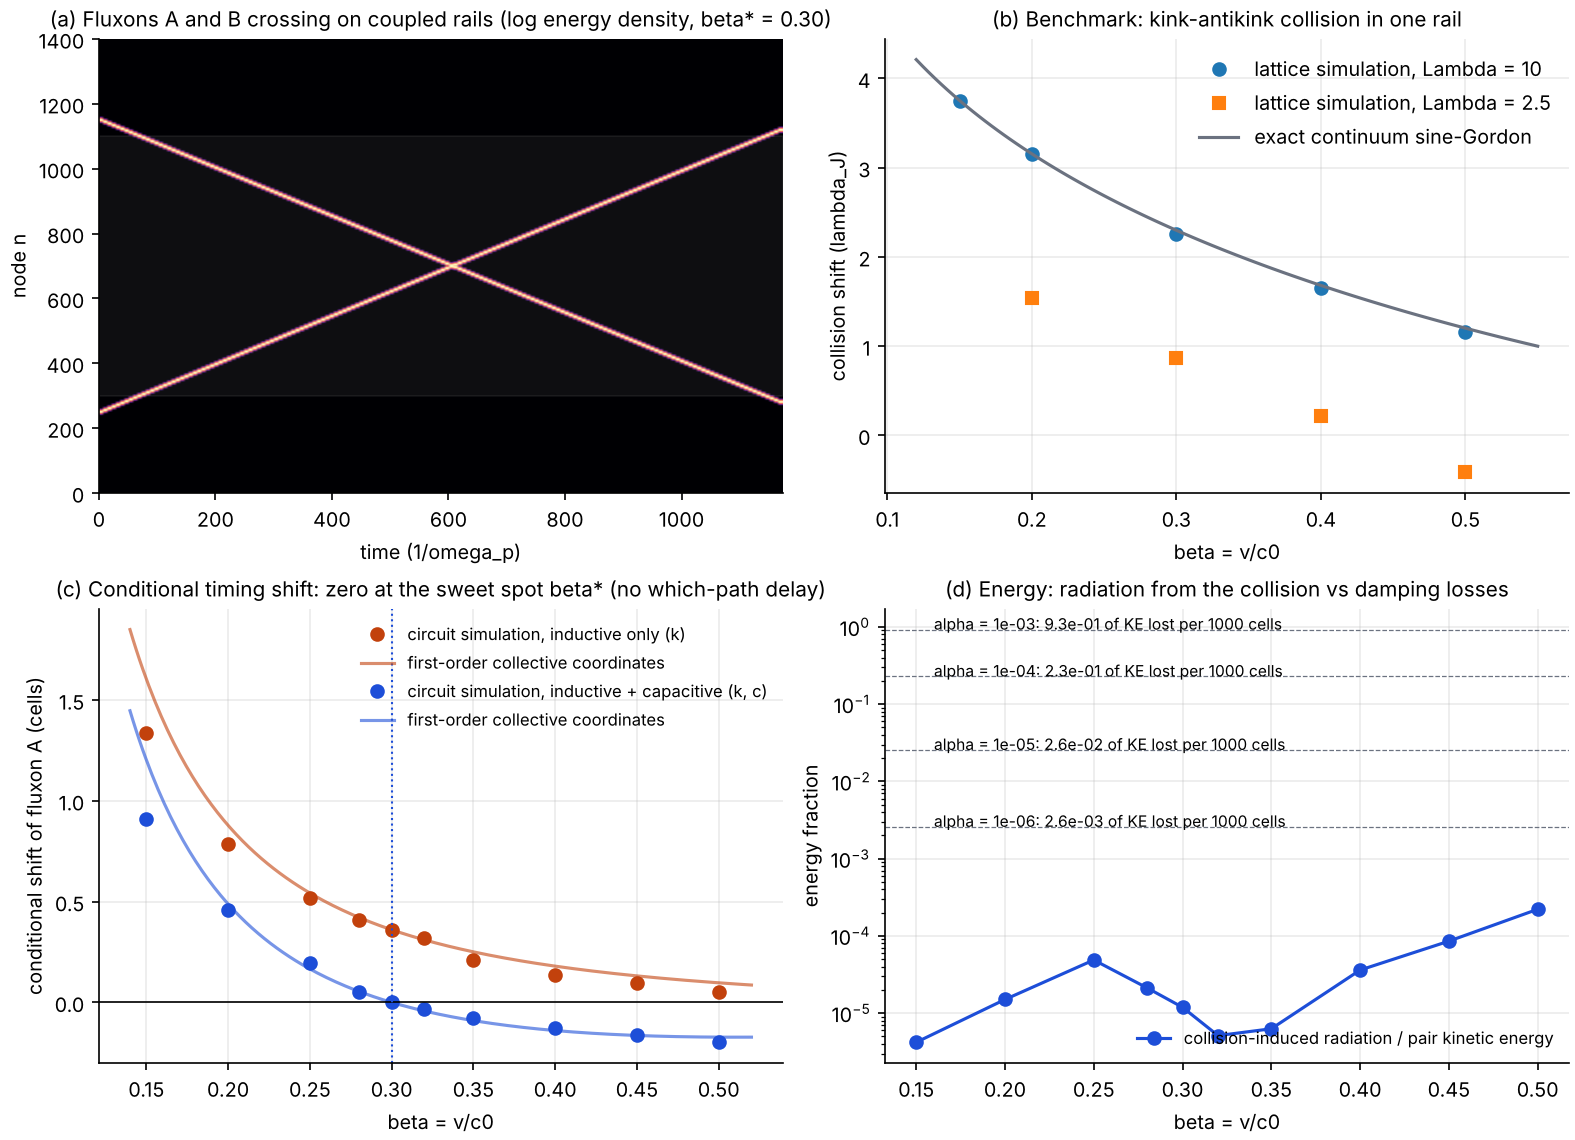
\includegraphics[width=0.64\textwidth]{../figures/fig01_classical_collision.png}
\caption{Milestone A, circuit simulations at the first-order design $\beta^*=0.30$. (a)~Energy density (log scale) of
fluxons A and B crossing on the coupled rails. (b)~Shift after a kink--antikink collision in one rail (units of
$\lambda_J$), lattice at $\Lambda=10$ and 2.5 against the exact continuum result. (c)~Conditional shift of fluxon A for
the inductive-only ($k$) and the mixed ($k$, $c$) coupler, circuit (points) and first-order theory (lines); the mixed
shift crosses zero at $\beta=0.302$. (d)~Magnitude of the collision-induced radiation relative to the pair kinetic
energy (mixed coupler) and damping loss per 1000 cells for $\alpha=10^{-6}$ to $10^{-3}$ (dashed).}
\label{fig:classical}
\end{figure*}

\subsection{Milestone B: quantum ballistic physics}
\label{sec:resB}
A single wavepacket ($\sigma_0=3$ cells, $\beta=0.3$) moves at 238.22 cells/ns against 238.43 cells/ns from
Eq.~\eqref{eq:disp} and spreads coherently to 45.93 cells against 45.94 cells analytically; the norm is conserved to
$2\ee{-13}$ (Fig.~\ref{fig:wavepacket}). The derived interaction agrees with the constrained relaxation of the circuit:
$-9.693$ against $-9.621$~GHz at contact (+0.76\%) and $-1.417$ against $-1.426$~GHz at a separation of 10 cells.

Figure~\ref{fig:joint} shows the sweet-spot collision at $\beta=0.30$ with the first-order coupler. Both fluxons are
transmitted (reflection $7.1\ee{-8}$), the motional Schmidt purity of the outgoing $\ket{11}$ state is 0.9999988
(Schmidt coefficients 0.9999994 and $5.9\ee{-7}$), and $|\omega|=0.9999989$. The mean conditional shift of fluxon A is
$-0.017$ cells. With an inductive-only coupler of the same $k$ the shift is $+0.339$ cells and $|\omega|=0.9997123$: the
which-path distinguishability $1-|\omega|$ falls from $2.9\ee{-4}$ to $1.1\ee{-6}$ when the capacitive coupler is
added, and the momentum-resolved conditional phase becomes flat around $k_0$.

Figure~\ref{fig:qc} compares 2D scattering, first order and the circuit at five speeds. The quantum mean shift crosses
zero at $\beta=0.2933$ and the circuit shift at 0.3020, within the 0.02 required by milestone B. At all ten points the
quantum shift differs from the classical limit of the same model by at most 8.9\% of the delay scale (the
inductive-coupler shift at that speed). For the mixed coupler the 2D phase is 3.3265, 3.2800, 3.2719, 3.2922 and
3.3341~rad (modulo $2\pi$) at $\beta=0.24$, 0.27, 0.30, 0.33 and 0.36, smallest near the design speed and 0.130~rad
above the first-order value $\pi$ at 0.30. For the inductive coupler it follows first order closely (1.5422 against
1.5708~rad at 0.30). An earlier milestone-B correspondence test used the single point where both scans had a shift
above 0.05 cells (5.8\%) and was replaced by these two tests over all ten points.

\begin{figure*}[t]
\centering
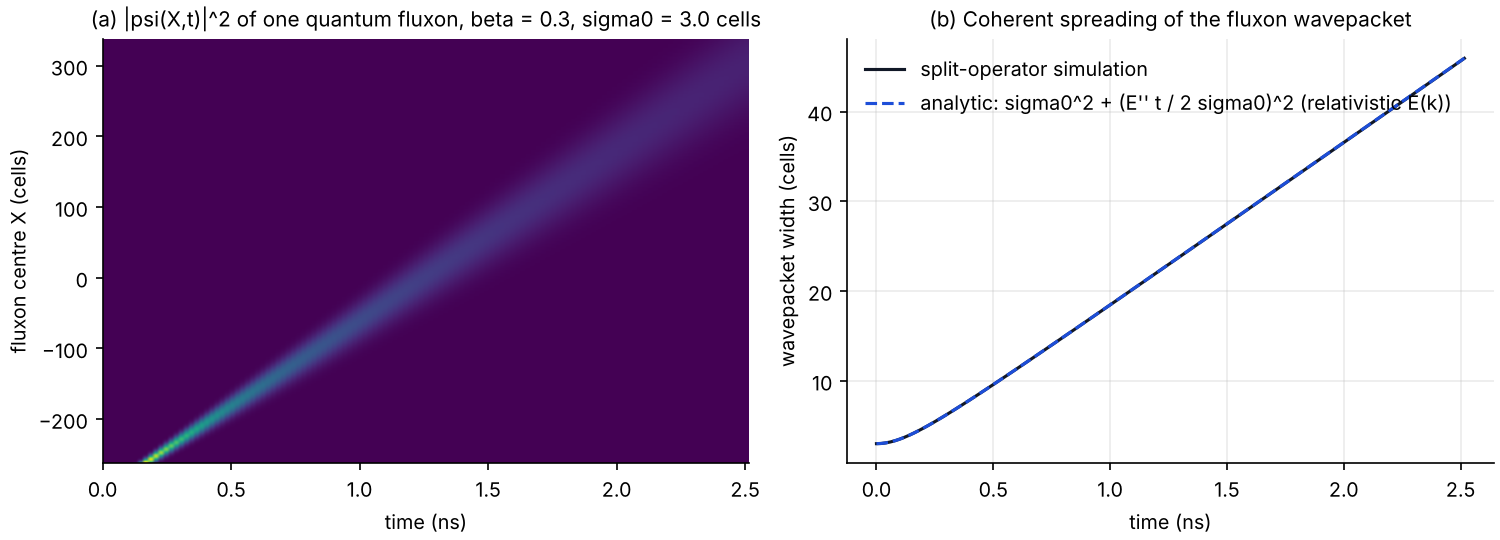
\includegraphics[width=0.56\textwidth]{../figures/fig02_single_wavepacket.png}
\caption{Milestone B: one quantum fluxon ($\beta=0.3$, $\sigma_0=3$ cells) propagated with the relativistic
dispersion~\eqref{eq:disp}. (a)~$|\psi(X,t)|^2$. (b)~Width from the split-operator simulation and the analytic spreading
law.}
\label{fig:wavepacket}
\end{figure*}

\begin{figure*}[t]
\centering
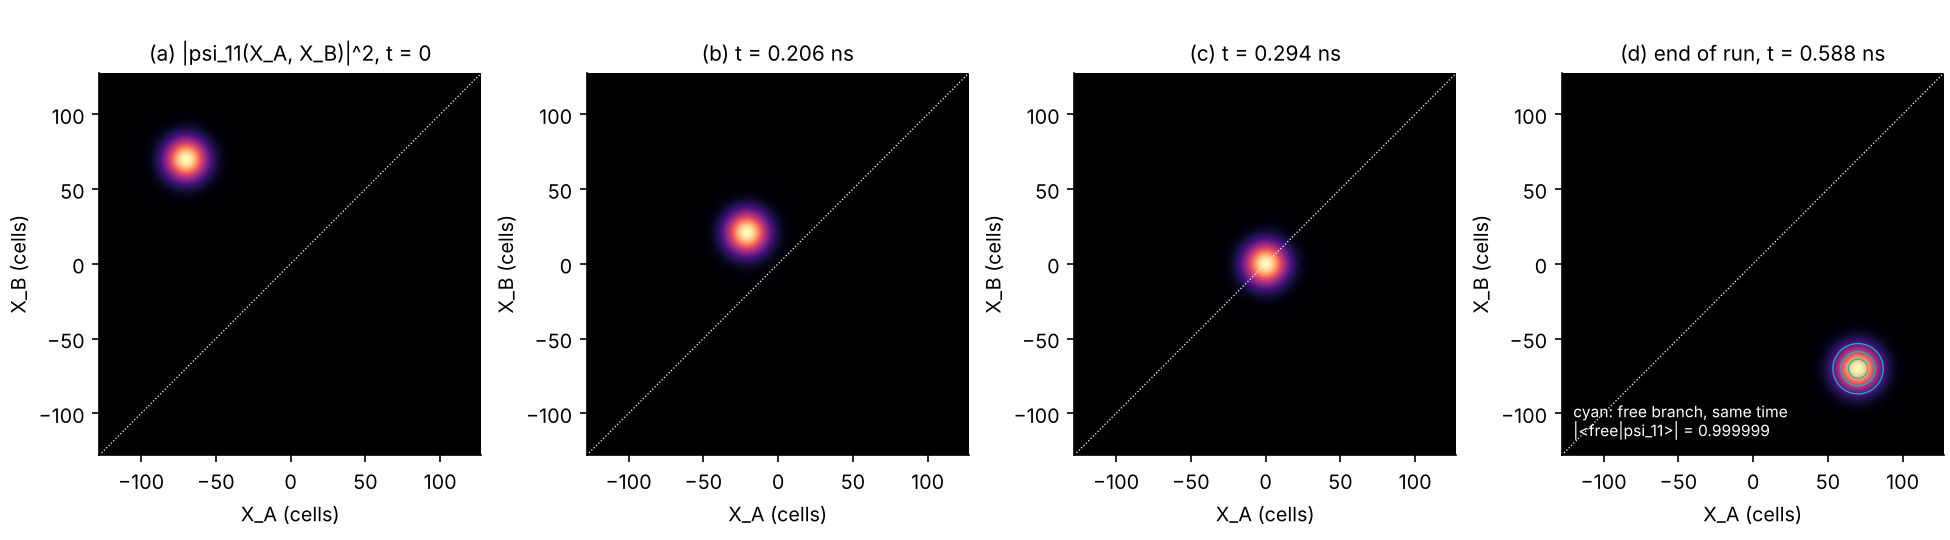
\includegraphics[width=0.88\textwidth]{../figures/fig03_joint_probability.png}\\[2pt]
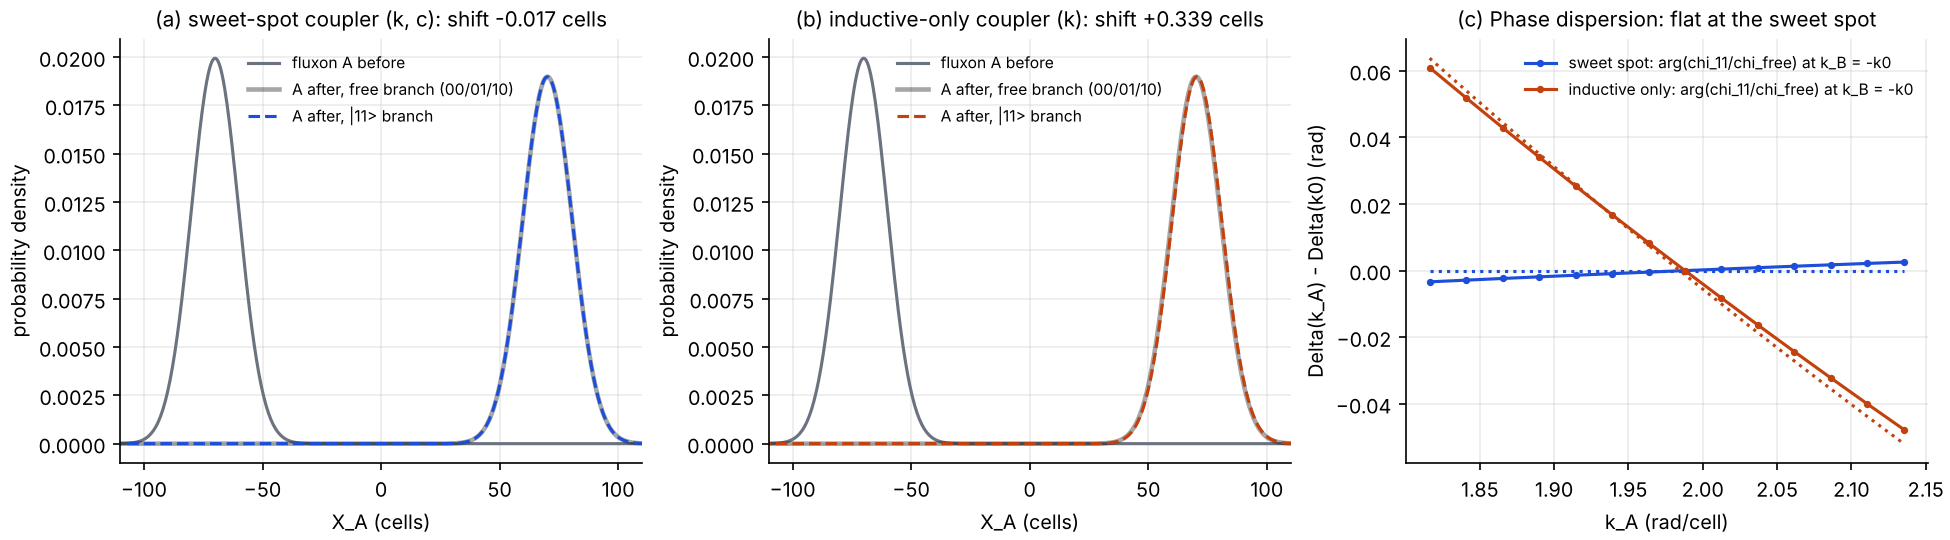
\includegraphics[width=0.88\textwidth]{../figures/fig04_scattering_before_after.png}
\caption{Sweet-spot collision at $\beta^*=0.30$ ($\sigma=10$ cells). Top, (a)--(d): joint probability
$|\psi_{11}(X_A,X_B)|^2$ at $t=0$, 0.206~ns, 0.294~ns and at the end of the run, $t=0.588$~ns, with the diagonal
$X_A=X_B$ dotted. In (d) the cyan contours show the free branch at the same time; the two overlap, with
$|\omega|=0.999999$. Bottom: (a), (b)~marginal of fluxon A before and after the collision for the free and
the $\ket{11}$ branch, with the sweet-spot coupler and an inductive-only coupler of the same $k$ (shifts $-0.017$ and
$+0.339$ cells). (c)~Momentum-resolved conditional phase $\arg(\chi_{11}/\chi_{\rm free})$ at $k_B=-k_0$, 2D (points)
and first order (dotted).}
\label{fig:joint}
\end{figure*}

\begin{figure*}[t]
\centering
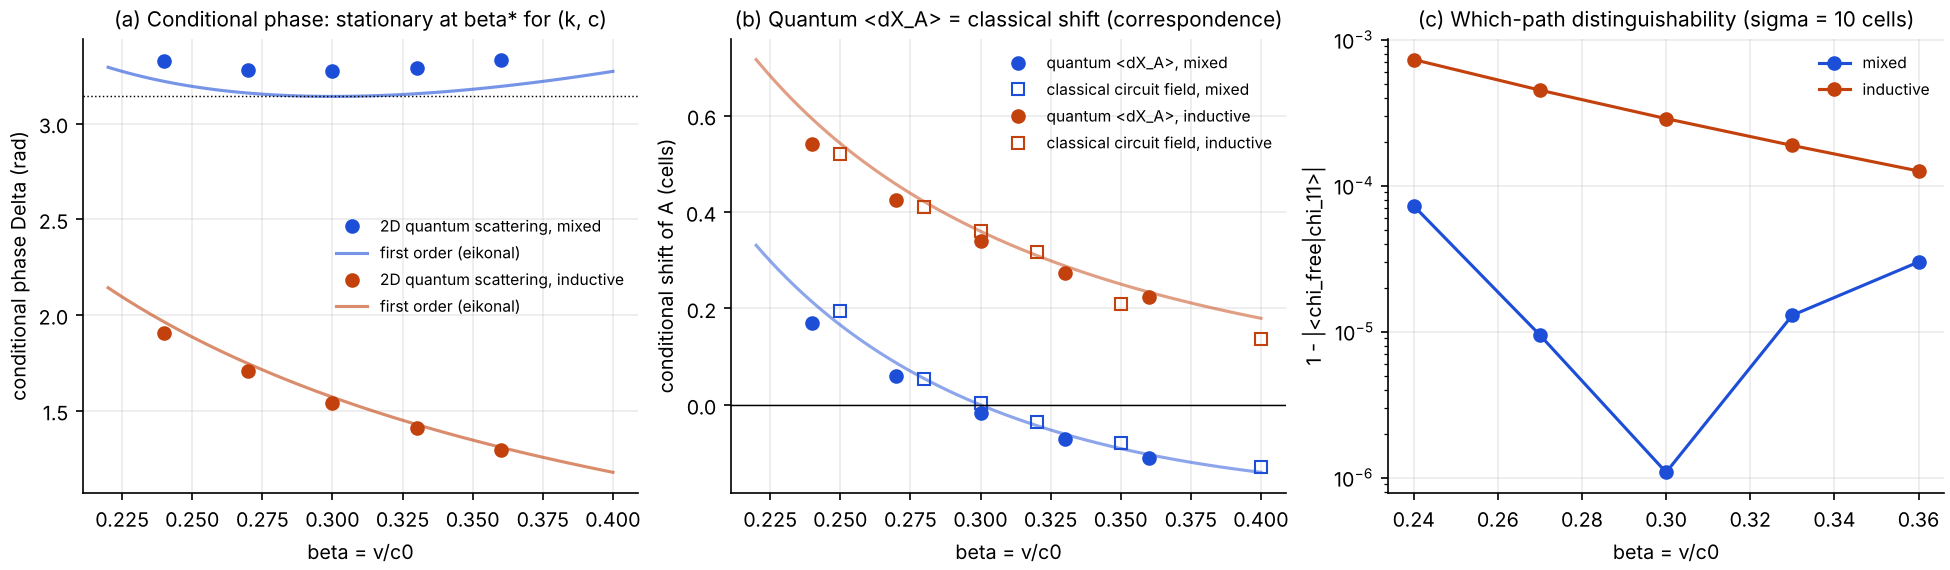
\includegraphics[width=0.88\textwidth]{../figures/fig09_quantum_vs_classical.png}
\caption{Quantum versus classical (first-order design for $\beta^*=0.30$). (a)~Conditional phase from 2D scattering
(points) and first order (lines) for the mixed and the inductive coupler; dotted line: $\pi$. (b)~Quantum mean shift
$\langle\Delta X_A\rangle$, classical circuit shift (open squares) and first-order shift (lines). (c)~Which-path
distinguishability $1-|\braket{\chi_{\rm free}|\chi_{11}}|$ for $\sigma=10$ cells.}
\label{fig:qc}
\end{figure*}

\subsection{Milestone C: the entangling gate}
\label{sec:resC}
Table~\ref{tab:gate} lists the logical metrics with the 2D-calibrated coupler. At $\beta^*=0.30$ the conditional phase
is 3.14325~rad modulo $2\pi$, $1.7\ee{-3}$~rad from $\pi$. From $\ket{+}\ket{+}$ the gate gives concurrence 0.9999995
and logical purity 0.9999998; the Bell fidelity and the CZ process fidelity are 0.9999994 (0.999999 to six decimals),
and the leakage is $6.2\ee{-8}$. The motional Schmidt purity is 0.9999989, so the entanglement is logical, not motional.
Ignoring the motion ($|\omega|$ set to 1) would give a process fidelity of 0.9999995, so the residual motional
distinguishability costs about $1.3\ee{-7}$ and most of the remaining error comes from the residual phase error. With
the coupler off the concurrence is $2.1\ee{-8}$ and the CZ process fidelity 0.49999999, as expected for the identity.

\begin{table}[t]
\centering\footnotesize
\caption{Logical metrics from exact 2D scattering with pure wavepackets and the 2D-calibrated coupler
(\file{C\_\allowbreak{}gate.\allowbreak{}json}: \file{gate\_\allowbreak{}pure}, \file{optimum\_\allowbreak{}validation.\allowbreak{}gate\_\allowbreak{}pure}, \file{control\_\allowbreak{}coupler\_\allowbreak{}off}). $\Delta$
is modulo $2\pi$; fidelities are after the best local $Z$ corrections.}
\label{tab:gate}
\setlength{\tabcolsep}{3.4pt}
\begin{tabular}{@{}lccc@{}}
\toprule
Quantity & $\beta^*=0.30$ & $\beta=0.45$ & coupler off\\
\midrule
$\Delta$ (rad) & 3.14325 & 3.14173 & $-2.9\ee{-14}$\\
$|\omega|$ & 0.9999997 & 0.99999991 & 0.99999996\\
leakage $1-p_{11}$ & $6.2\ee{-8}$ & $1.1\ee{-7}$ & $4.2\ee{-8}$\\
concurrence & 0.9999995 & 0.99999997 & $2.1\ee{-8}$\\
entanglement of formation & 0.9999993 & 0.99999996 & $6.0\ee{-15}$\\
entropy of qubit A (bit) & 0.9999995 & 0.999999997 & $1.5\ee{-7}$\\
logical purity & 0.9999998 & 0.99999997 & 0.99999998\\
Bell fidelity & 0.9999994 & 0.99999996 & 0.49999999\\
CZ process fidelity & 0.9999994 & 0.99999996 & 0.49999999\\
CZ average gate fidelity & 0.9999995 & 0.99999997 & 0.59999999\\
distinguishability $D$ & $3.0\ee{-7}$ & $3.4\ee{-8}$ & $2.1\ee{-8}$\\
motional purity & 0.9999989 & -- & --\\
\bottomrule
\end{tabular}
\end{table}

\emph{Thermal launch and speed mismatch.} The launch-speed spread is evaluated with the first-order
phase~\eqref{eq:Delta}, averaged over independent Gaussian speed distributions of the two launchers, with each coupler
scaled to give $\pi$ at $\beta=0.30$. At 20~mK (spread 7.1\%) the CZ error $1-F_{\rm avg}$ is $1.2\ee{-5}$ at the
sweet spot and $3.8\ee{-3}$ with an inductive-only coupler; from 5 to 100~mK the sweet-spot error grows from
$1.0\ee{-6}$ to $2.9\ee{-4}$ and the inductive-only error from $9.4\ee{-4}$ to $2.0\ee{-2}$ (Fig.~\ref{fig:sens}a). A
systematic mismatch $|\beta_B-\beta_A|=0.05$ costs at most $5.6\ee{-6}$ at the sweet spot and $4.1\ee{-3}$ without it.
The phase model was checked against 2D scattering with $\beta_A=0.30$: the 2D and model phases are 3.143 and 3.145~rad
for $\beta_B=0.27$ and 3.143 and 3.138~rad for $\beta_B=0.33$.

\emph{Coupling strength and timing.} Scaling $k$ and $c$ by $s=0.25$, 0.5, 0.75, 1 and 1.25 gives $\Delta=0.764$,
1.542, 2.335, 3.143 and 3.968~rad and concurrences 0.373, 0.697, 0.920, 0.9999995 and 0.916 (Figs.~\ref{fig:strength}
and~\ref{fig:conc}). The phase lies close to the rescaled first-order line, and the concurrences equal $|\sin(\Delta/2)|$
to three decimals, as for a pure logical state. An uncalibrated strength error of $\pm5$\% gives a CZ error of
$1.3\ee{-3}$ and $\pm10$\% gives $5.0\ee{-3}$ (Fig.~\ref{fig:sens}c), so the coupler needs calibration, a flux-tunable
$L_s$ or speed retuning. A launch-time mismatch moves the meeting point along the coupler. With a 60-cell plateau, 2D
scattering gives $F_{\rm avg}=0.99991$ for 0.1~ns (meeting point moved by 11.9 cells), 0.9885 for 0.2~ns (23.8 cells),
0.849 for 0.3~ns and 0.672 for 0.38~ns (45.3 cells), and the first-order model follows these points
(Fig.~\ref{fig:timing}). Longer plateaus move the onset of the error to larger mismatch, and for the 100-cell plateau
and 10~ps rms jitter of the budget the timing term evaluates to zero.

\begin{figure*}[t]
\centering
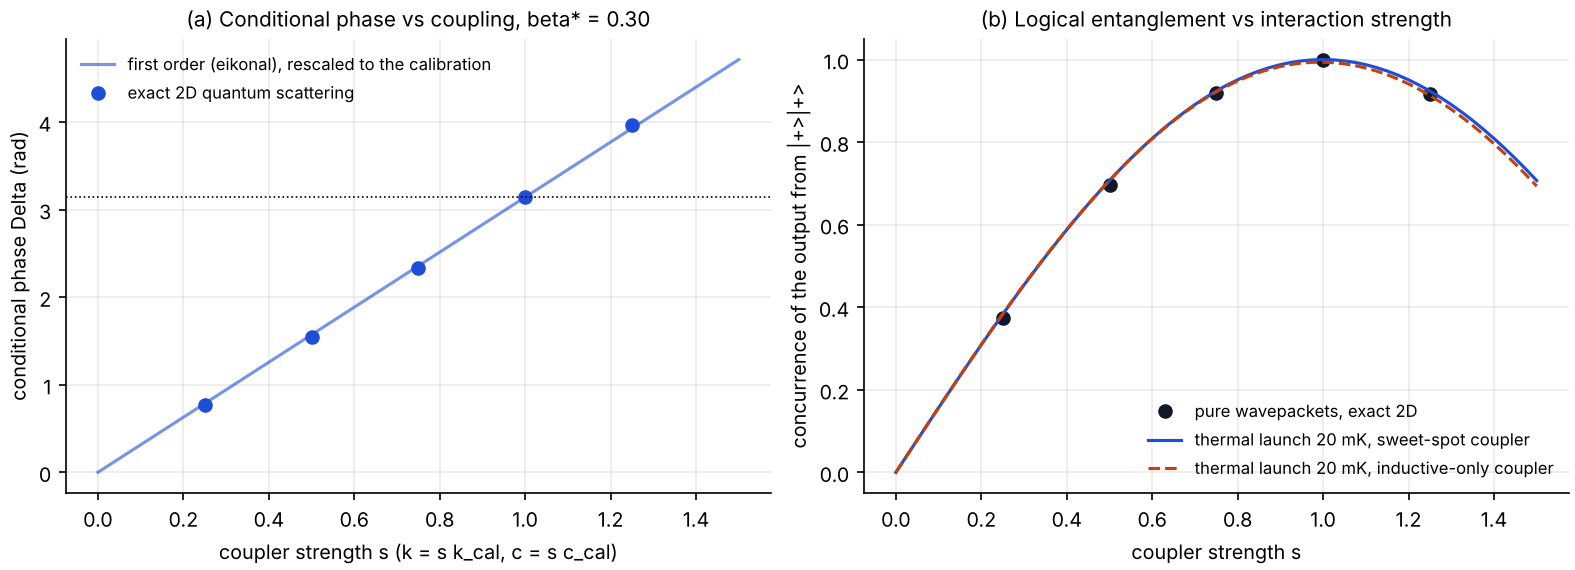
\includegraphics[width=0.62\textwidth]{../figures/fig05_phase_vs_coupling.png}
\caption{Milestone C at $\beta^*=0.30$. (a)~Conditional phase versus coupler strength $s$ ($k=s\,k_{\rm cal}$,
$c=s\,c_{\rm cal}$): exact 2D scattering (points) and first order rescaled to the calibration (line); dotted line:
$\pi$. (b)~Concurrence of the output from $\ket{+}\ket{+}$: exact 2D for pure wavepackets (points) and first-order
model for a 20~mK thermal launch with the sweet-spot (solid) and the inductive-only coupler (dashed).}
\label{fig:strength}
\end{figure*}

\begin{figure}[t]
\centering
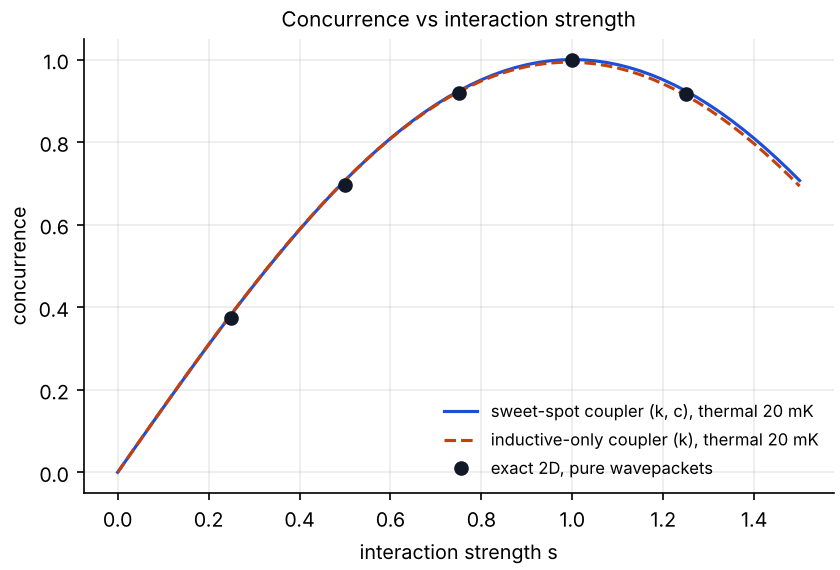
\includegraphics[width=0.88\columnwidth]{../figures/fig06_concurrence_vs_strength.png}
\caption{Concurrence versus interaction strength $s$, the quantity of Fig.~\ref{fig:strength}(b) in one panel.}
\label{fig:conc}
\end{figure}

\begin{figure}[t]
\centering
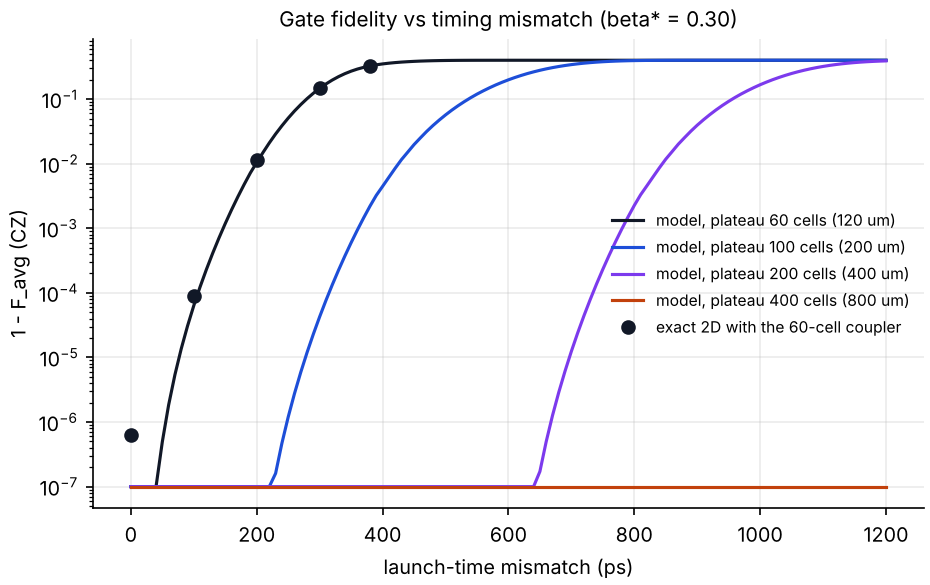
\includegraphics[width=0.96\columnwidth]{../figures/fig07_fidelity_vs_timing.png}
\caption{CZ error versus launch-time mismatch at $\beta^*=0.30$: exact 2D scattering with a 60-cell plateau (points)
and the first-order model for 60-, 100-, 200- and 400-cell plateaus (lines, floored at $10^{-7}$ for display).}
\label{fig:timing}
\end{figure}

\begin{figure*}[t]
\centering
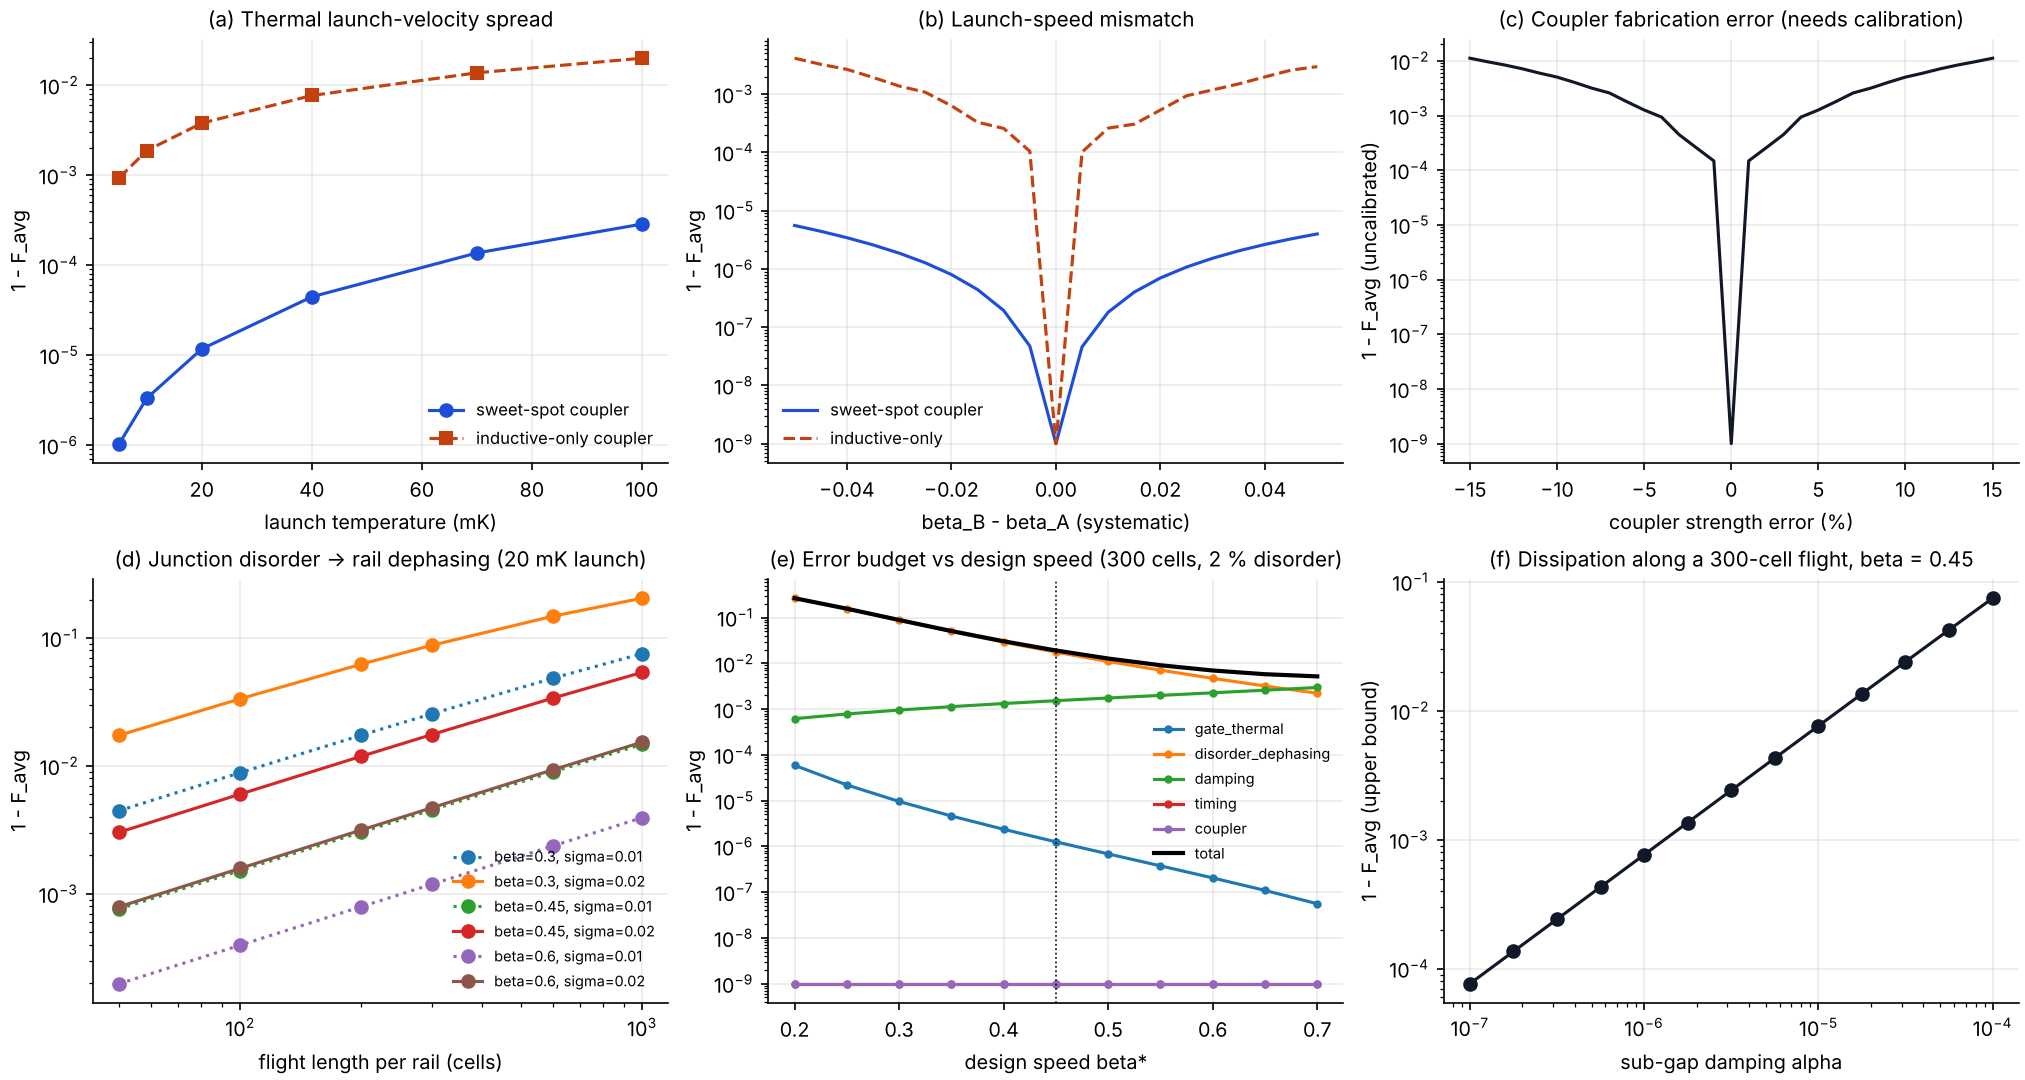
\includegraphics[width=0.90\textwidth]{../figures/fig08_noise_loss_sensitivity.png}
\caption{Sensitivity of the gate. (a)~CZ error versus launch temperature, sweet-spot and inductive-only coupler
($\beta=0.30$). (b)~Systematic launch-speed mismatch. (c)~Uncalibrated coupler-strength error. (d)~Dephasing from
junction disorder versus flight length per rail, for $\beta=0.3$, 0.45, 0.6 and disorder of 1\% and 2\% (20~mK
launch). (e)~Error budget versus design speed (300 cells, 2\% disorder); the dotted line marks the operating point
$\beta=0.45$, and points above it lie outside the range where the effective model was checked against the circuit.
(f)~Damping contribution along a 300-cell flight at $\beta=0.45$ (upper bound). Zero values are plotted at a
$10^{-9}$ floor in (b), (c) and (e).}
\label{fig:sens}
\end{figure*}

\subsection{Calibration history}
\label{sec:calib}
At $\beta^*=0.30$ the first-order design gives $\Delta=3.2719$~rad and $\ud\Delta/\ud\beta=0.229$; two corrections
bring them to 3.1432~rad and 0.0020 (Table~\ref{tab:calib}). At $\beta=0.45$ the first-order design is closer, and the
calibrated coupler reaches $\Delta=3.14173$~rad ($1.3\ee{-4}$~rad from $\pi$) and $\ud\Delta/\ud\beta=2.2\ee{-5}$.

\begin{table}[t]
\centering\footnotesize
\caption{Calibration of the coupler on exact 2D scattering. Iteration 0 is the first-order design, and $\Delta$ is
modulo $2\pi$.
Source: \file{C\_\allowbreak{}gate.\allowbreak{}json}, keys \file{calibration\_\allowbreak{}reference.\allowbreak{}history} and
\file{optimum\_\allowbreak{}validation.\allowbreak{}calibration}.}
\label{tab:calib}
\setlength{\tabcolsep}{4pt}
\begin{tabular}{@{}ccccc@{}}
\toprule
iteration & $k$ & $c$ & $\Delta$ (rad) & $\ud\Delta/\ud\beta$\\
\midrule
\multicolumn{5}{@{}l}{$\beta^*=0.30$}\\
0 & 0.012077 & 0.13421 & 3.27190 & 0.229\\
1 & 0.011841 & 0.12571 & 3.12516 & $-0.0139$\\
2 & 0.011888 & 0.12659 & 3.14325 & 0.0020\\
\multicolumn{5}{@{}l}{$\beta=0.45$}\\
0 & 0.018113 & 0.089474 & 3.20899 & 0.0139\\
1 & 0.017760 & 0.087377 & 3.13844 & $-3.0\ee{-5}$\\
2 & 0.017778 & 0.087467 & 3.14173 & $2.2\ee{-5}$\\
\bottomrule
\end{tabular}
\end{table}

\section{Optimisation and error budget}
\label{sec:budget}

\emph{Error channels.} The budget adds five contributions to the CZ error $1-F_{\rm avg}$, each for a coupler
redesigned to have its sweet spot at the operating speed. (i) Thermal launch, as in Sec.~\ref{sec:resC}. (ii) Disorder:
random cell errors of $E_J$, $E_L$ and $C$ (relative rms $\sigma_J$, $\sigma_L$, $\sigma_C$) change the energy of a
passing kink through its Josephson, inductive and kinetic shares, $4\Lambda/\gamma$, $4\Lambda\gamma$ and
$4\Lambda\gamma\beta^2$ (units of $E_J$), so one cell adds a random phase of rms $\sigma_{\rm cell}=2\pi E_Jw/v$ with
$w=[(4\Lambda\sigma_J/\gamma)^2+(4\Lambda\gamma\sigma_L)^2+(4\Lambda\gamma\beta^2\sigma_C)^2]^{1/2}$ ($E_J$ in GHz, $v$
in cells/ns). The two rails of a qubit, $N$ cells each, then differ by a static phase of rms
$\Phi=(2N)^{1/2}\sigma_{\rm cell}$. Its static part is a calibratable single-qubit phase, but it scales as $1/v$, so the
launch-speed spread $s$ turns it into dephasing with probability $p_{\rm dis}=1-(1+\Phi^2s^2)^{-1/2}$. (iii) Damping:
the energy lost along the flight, $\alpha v(8\gamma/\Lambda)N$ in units of $E_J$, is counted in plasma quanta, each
treated as which-rail information (an upper bound). (iv) Timing: the rms meeting-point offset from the jitter of the two
launchers, averaged over the wavepacket overlap on a plateau with cosine tapers. (v) Coupler: an uncalibrated strength
error $\epsilon$ gives $\Delta=\pi(1+\epsilon)$. Dephasing probabilities are converted to CZ errors through
Eq.~\eqref{eq:schur}. The defaults are 300 cells per rail, 2\% disorder in $E_J$, $E_L$ and $C$, a 20~mK launch,
$\alpha=2\ee{-6}$, 10~ps jitter and a 100-cell plateau.

\emph{Scan and optimum.} Table~\ref{tab:budget} and Fig.~\ref{fig:sens}(e) give the budget from $\beta=0.20$ to 0.70.
Disorder dephasing dominates at every speed in the validated range and falls roughly as $\beta^{-4}$, from 8.8\% at
$\beta=0.30$ to 1.8\% at 0.45; the thermal gate term stays below $10^{-4}$, and damping grows slowly with speed. The
optimiser is restricted to $\beta\le0.45$, where the collective-coordinate model agrees with the circuit, and picks
$\beta=0.45$. Faster fluxons would reduce the disorder term further but need a full-circuit quantum treatment, so the
rows above 0.45 are not used. At the optimum the total is 1.9\% ($1.913\ee{-2}$): disorder $1.76\ee{-2}$ (rms rail phase
difference 4.99~rad, dephasing probability 2.2\%, launch spread 4.3\%), damping $1.53\ee{-3}$, thermal gate
$1.26\ee{-6}$, timing and coupler 0. The scan lists a thermal term of $9.6\ee{-6}$ at $\beta=0.30$, not the $1.2\ee{-5}$ of
Sec.~\ref{sec:resC}, because it uses the first-order coupler, not the 2D-calibrated one.

\begin{table}[t]
\centering\footnotesize
\caption{Error budget versus design speed (\file{C\_\allowbreak{}gate.\allowbreak{}json}, \file{budget\_\allowbreak{}scan\_\allowbreak{}default}); 300 cells per rail,
2\% disorder, 20~mK, $\alpha=2\ee{-6}$, 10~ps jitter, 100-cell plateau. Timing and coupler terms are 0 in every row;
$\Phi$ is the rms rail phase difference. Rows marked $^\dagger$ lie outside the validated range of the effective model
and are excluded from the optimisation.}
\label{tab:budget}
\setlength{\tabcolsep}{2.5pt}
\begin{tabular}{@{}cccccc@{}}
\toprule
$\beta$ & thermal & disorder & damping & total & $\Phi$ (rad)\\
\midrule
0.20 & $5.9\ee{-5}$ & 0.265 & $6.2\ee{-4}$ & 0.266 & 11.0\\
0.25 & $2.2\ee{-5}$ & 0.156 & $7.8\ee{-4}$ & 0.157 & 8.78\\
0.30 & $9.6\ee{-6}$ & 0.0878 & $9.5\ee{-4}$ & 0.0888 & 7.34\\
0.35 & $4.6\ee{-6}$ & 0.0498 & $1.13\ee{-3}$ & 0.0509 & 6.31\\
0.40 & $2.4\ee{-6}$ & 0.0291 & $1.32\ee{-3}$ & 0.0304 & 5.56\\
\textbf{0.45} & $\mathbf{1.3\ee{-6}}$ & \textbf{0.0176} & $\mathbf{1.53\ee{-3}}$ & \textbf{0.0191} & \textbf{4.99}\\
0.50$^\dagger$ & $6.9\ee{-7}$ & 0.0110 & $1.75\ee{-3}$ & 0.0128 & 4.56\\
0.55$^\dagger$ & $3.8\ee{-7}$ & 0.00711 & $2.00\ee{-3}$ & 0.00910 & 4.24\\
0.60$^\dagger$ & $2.0\ee{-7}$ & 0.00471 & $2.28\ee{-3}$ & 0.00699 & 4.00\\
0.65$^\dagger$ & $1.1\ee{-7}$ & 0.00320 & $2.59\ee{-3}$ & 0.00580 & 3.86\\
0.70$^\dagger$ & $5.6\ee{-8}$ & 0.00223 & $2.97\ee{-3}$ & 0.00520 & 3.80\\
\bottomrule
\end{tabular}
\end{table}

\emph{Validation at the optimum.} In the circuit, the conditional shift of fluxon A for the coupler redesigned for
$\beta=0.45$ is 0.0674, 0.0308, 0.0028, $-0.0185$ and $-0.0366$ cells at $\beta=0.39$, 0.42, 0.45, 0.48 and 0.51
(first order 0.0716, 0.0306, 0, $-0.0226$, $-0.0390$) and crosses zero at $\beta=0.4539$. In exact 2D scattering,
calibration from the first-order values $k=0.01811$, $c=0.08947$ gives $k=0.01778$, $c=0.0875$ (Table~\ref{tab:calib}),
and the calibrated gate has CZ process fidelity 0.99999996, concurrence 0.99999997 and leakage $1.1\ee{-7}$
(Table~\ref{tab:gate}). The budget itself is evaluated with the first-order coupler of the scan.

\emph{What a sub-1\% gate needs.} At $\beta=0.45$ a 362-cell flight takes 1.01~ns at 357.6 cells/ns, far shorter than
the microsecond coherence times reported for vortex qubits, so dephasing from disorder, not decoherence in flight,
limits the gate. Table~\ref{tab:disorder} gives the total for three disorder levels and three flight lengths. A total
below 1\% requires junction disorder of 1\% or less (0.73\% over the full 362-cell rows) or flights of at most 150
cells at 2\% disorder (0.97\%). At 0.5\% disorder the total is 0.13--0.32\%. Lower damping would reduce the remaining
$1.5\ee{-3}$ term. None of these conditions has been demonstrated.

\begin{table}[t]
\centering\footnotesize
\caption{Total CZ error at $\beta=0.45$ versus junction disorder and flight length per rail (\file{D\_\allowbreak{}feasibility.\allowbreak{}json},
\file{constraints.\allowbreak{}disorder\_\allowbreak{}length\_\allowbreak{}scan}); other assumptions as in Table~\ref{tab:budget}.}
\label{tab:disorder}
\begin{tabular}{@{}cccc@{}}
\toprule
disorder & 150 cells & 300 cells & 362 cells\\
\midrule
0.5\% & 0.13\% & 0.27\% & 0.32\%\\
1\% & 0.30\% & 0.61\% & 0.73\%\\
2\% & 0.97\% & 1.91\% & 2.29\%\\
\bottomrule
\end{tabular}
\end{table}

\section{Device design}
\label{sec:device}

\emph{Architecture and netlist.} The design uses the optimum with its 2D-calibrated coupler ($\beta=0.45$,
$k=0.01778$, $c=0.0875$). Each of the six rows has 362 cells (724~$\mu$m). Along the path of fluxon A the sections are
injection (10 cells), accelerator (40), preparation beam splitter (41), gap (20), taper (40), coupler plateau (100),
taper (40), gap (20), analysis beam splitter (41) and detection (10), and qubit B mirrors this. All junctions come
from one oxidation ($J_c\approx2.1~\mu$A/$\mu$m$^2$, 50~fF/$\mu$m$^2$). The rail junctions have $I_c=80.5$~nA and
0.038~$\mu$m$^2$ (1.92~fF) with a 0.50~fF node shunt, reduced to 0.29~fF on the coupler plateaus, so the node capacitance
is 2.42~fF outside and 2.21~fF inside the couplers, where the series inductance is 0.642~nH. The middle-rail junctions
have $E_{J,M}=25.3$~GHz and 0.024~$\mu$m$^2$ (1.21~fF) with a 0.31~fF island shunt, which gives $E_{C,M}=12.7$~GHz and
$E_S=1.10$~GHz. The coupler strips have $L_s=11.6$~pH and the coupling capacitors $C_c=0.21$~fF. The injection junction
has 161~nA (0.077~$\mu$m$^2$), and its coherent operation is unresolved. The shunts are to come from the geometric node,
line and island capacitance plus a trim, set by electromagnetic extraction. The complete netlist
(\file{circuits/\allowbreak{}qbfx2\_\allowbreak{}netlist.\allowbreak{}cir}) has 8082 elements: 2172 rail junctions and 2172 node shunt capacitors (junction
model $I_c=80.5$~nA, $C_j=1.92$~fF, shunt 0.50~fF), 2166 granular-Al inductors, 540 coupler-strip inductors and 540
coupling capacitors (gate and dummy couplers), 160 middle-rail junctions with 160 island shunt capacitors ($C_j=1.21$~fF,
shunt 0.31~fF), 4 injector junctions with 4 pulse sources, 160 accelerator bias sources and 4 catcher-loop inductors. A
parser finds 2877 nodes and no isolated node.

\emph{Layout.} The preliminary layout (\file{circuits/\allowbreak{}qbfx2\_\allowbreak{}layout.\allowbreak{}gds}, Figs.~\ref{fig:schematic}e
and~\ref{fig:layout}) measures $844\times182~\mu$m$^2$, with six rows (row opening 8~$\mu$m, strip 2~$\mu$m) at a
2~$\mu$m pitch. Rail junctions are $0.2\times0.1917~\mu$m$^2$ overlaps (0.0383~$\mu$m$^2$) and middle-rail junctions
$0.18\times0.1348~\mu$m$^2$ (0.0243~$\mu$m$^2$); the coupler spans 360~$\mu$m and each beam splitter 82~$\mu$m.
Coupling-capacitor crossovers are drawn on all three couplers (540), whereas the node and island shunts are not drawn.
The layout has no design-rule check and no electromagnetic extraction of $k$, $c$, $E_S$ and the shunts, and the
crossover dielectric of the coupling capacitors is an extra, unverified process step, so it is not fabrication-ready.
The fabrication notes assume high-resistivity Si with a 150~nm Nb ground plane, Al/AlOx/Al double-angle junctions,
20~nm granular-Al inductors and 0.4~$\mu$m thin-Al coupler strips.

\begin{figure*}[t]
\centering
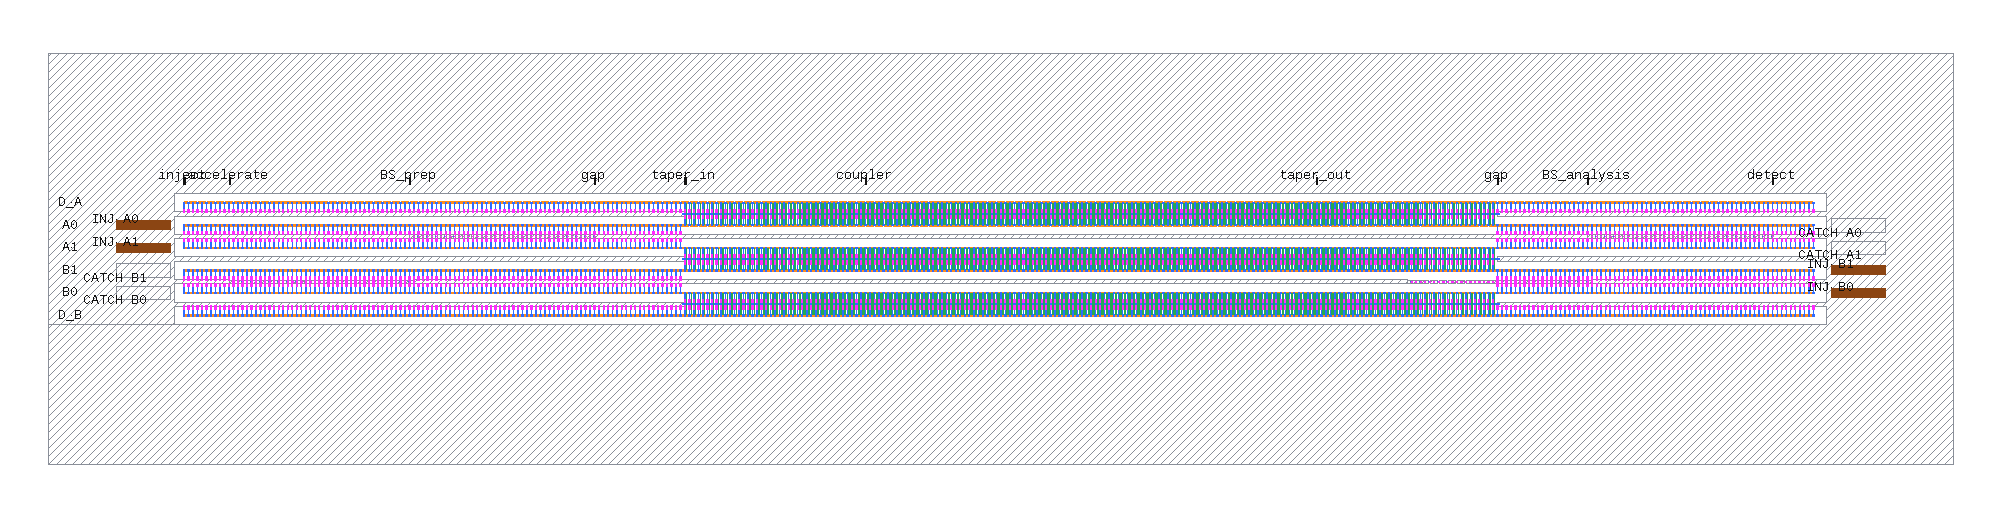
\includegraphics[width=0.92\textwidth]{../circuits/layout_overview.png}
\caption{Preliminary layout ($844\times182~\mu$m$^2$, not fabrication-ready). Rows from top to bottom: $D_A$, $A0$,
$A1$, $B1$, $B0$, $D_B$; labels mark the injection, accelerator, beam-splitter, gap, taper, coupler and detection
sections. The injectors (INJ) of qubit A are on the left and those of qubit B on the right, opposite the catchers
(CATCH) of the other qubit; the hatched area is the ground plane.}
\label{fig:layout}
\end{figure*}

\emph{Energy accounting.} Kinetic-energy retention was evaluated on the circuit model, with reference runs (free
rails, single fluxons) that separate the launch transient, the coupler traversal and the collision
(Fig.~\ref{fig:energy}). Without damping the gate (couplers + collision) retains 0.99998 of the kinetic energy at
$\beta=0.30$ and 0.99997 at 0.45. Coupler traversal costs $6.3\ee{-6}$ and $2.4\ee{-5}$, the collision $1.1\ee{-5}$ and
$3.3\ee{-6}$. Launch transient and flight lose a further $1.2\ee{-3}$ and $8.2\ee{-4}$, so the whole flight retains
0.99877 and 0.99916. With damping the flight loss at $\beta=0.45$ grows to $2.3\ee{-3}$, 1.5\% and 14\% for
$\alpha=10^{-6}$, $10^{-5}$ and $10^{-4}$ ($3.5\ee{-3}$, 2.4\% and 21\% at 0.30). For $\alpha\ge10^{-5}$ the
decomposition becomes unreliable at the $10^{-5}$--$10^{-4}$ level, with some gate retentions slightly above 1 (up to
1.00036). This energy test was redefined after the first results. It first divided the simulated outgoing kinetic
energy by the formula value $E_0(\gamma-1)$, and because the lattice kink starts slightly below that value a 0.5\% loss
appeared. With simulated values on both sides the whole-flight retention at $\beta=0.30$, 99.877\%, still failed the
$>99.9$\% criterion because of the launch transient (0.08--0.12\%). The test now applies to the gate, and both numbers
are reported. Braking and the energy per operation are given with companion 4 (Sec.~\ref{sec:companions}).

\begin{figure*}[t]
\centering
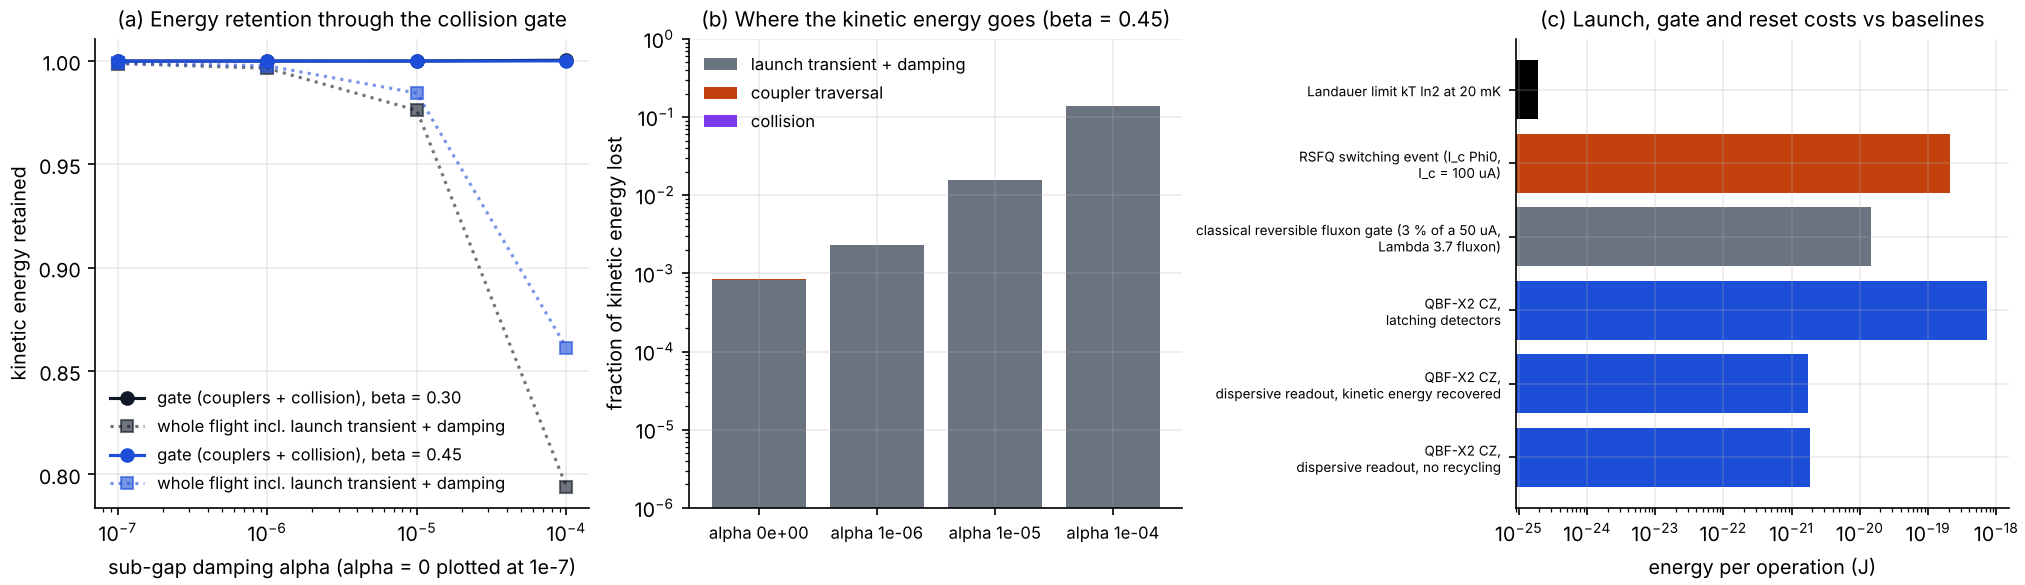
\includegraphics[width=0.88\textwidth]{../figures/fig10_energy_budget.png}
\caption{Energy accounting. (a)~Kinetic energy retained by the gate (couplers + collision, solid) and over the whole
flight including launch transient and damping (dotted), versus damping $\alpha$ ($\alpha=0$ plotted at $10^{-7}$), for
$\beta=0.30$ and 0.45. (b)~Where the kinetic energy goes at $\beta=0.45$. (c)~Estimated on-chip energy per operation of
QBF-X2 variants and baselines (companion 4), excluding control electronics, refrigeration and amplifiers.}
\label{fig:energy}
\end{figure*}

\emph{Cryogenic requirements.} A test needs a dilution refrigerator at 20~mK or below with $\mu$-metal and
superconducting shielding, an IR-tight sample box against quasiparticles and Cu quasiparticle traps near the
injectors; fast injector lines with rise time $\le20$~ps and a relative A--B launch timing $\le10$~ps (from on-chip
SFQ clocking or cryo-CMOS pulse generators); dc lines for the accelerators and the beam-splitter gate electrodes; and
catcher-loop resonators on a feedline read through a JPA or TWPA in single shot.

\emph{Staged measurement protocol.} The proposed experiment goes from classical to quantum tests:
(1)~single-rail transit, time of flight versus accelerator bias (speed, effective mass, damping); (2)~velocity
statistics, the time-of-flight histogram compared with the thermal launch spread; (3)~beam splitter and router,
Mach--Zehnder fringes versus gate voltage ($E_S$, splitting angle, contrast target $\ge0.99$); (4)~dual-rail coherence,
Ramsey-type interferometry with variable delay lines, a direct test of the disorder budget; (5)~classical sweet spot,
with only $A1$ and $B1$ occupied the arrival-time shift of fluxon A versus speed should cross zero at $v^*$, a
low-risk test of the key physics; (6)~conditional phase, A in $\ket{+}$ and B in $\ket{0}$ or $\ket{1}$, $\Delta$ from
the difference of A's Mach--Zehnder phases, target $\pi$ at $v^*$; (7)~entanglement, two-qubit tomography from
$\ket{+}\ket{+}$, Bell fidelity and a CHSH test; (8)~energy, time of flight before and after the gate and the braking
efficiency. Milestone D would change with a coherent single-fluxon injector with thermal-limited speed spread and
$\le10$~ps timing, a junction disorder of $\le1$\% across the 2,336 junctions of the chip (2172 rail, 160
middle-rail and 4 injection junctions, about 1,170 per qubit), electromagnetic extraction of $k$, $c$, $E_S$ with a DRC-clean layout, and a measured $\alpha\le10^{-6}$ at
20~mK.

\section{Companion devices}
\label{sec:companions}

Five companion devices were simulated with the same code, one simulation each (Fig.~\ref{fig:companions}).

\emph{1. Two-vortex Bell-pair chip.} Two independently addressed vortex qubits of the QFX-1 design idle at their double
sweet spots ($f_{01}=3.208$ and 3.608~GHz) and are coupled through an inductance $L_s=5$~pH ($J=18.9$~MHz). A
20~ns $\pi$ pulse and a 6.6~ns resonant exchange pulse produce a Bell pair. Including the dephasing of the pulsed qubit
while it is off its sweet spot ($7.8\ee{5}$~s$^{-1}$), the Bell fidelity is 0.9882, 0.9956 and 0.9976 for $T_1=5$, 20 and
100~$\mu$s (0.9981 without decay), with leakage below $10^{-12}$. The $T_1$ values are assumptions bracketing the reported range, and an
addressable entangled two-vortex processor was not found in the literature searched \cite{Nambisan2026}.

\emph{2. Coherent ballistic fluxon router.} A flying fluxon is split by a phase-slip beam splitter (here
$E_{J,M}/E_{C,M}=2$, $E_S=0.690$~GHz, 64.8 cells at $\beta=0.45$), carried on two ladder rows and recombined. The
Aharonov--Casher phase $\chi$ set by a gate voltage selects the exit row (row 1 with probability 0.99973 for $\chi=0$,
row 0 for $\chi=\pi$). The Mach--Zehnder fringe contrast is 1.0000 for a single speed, 0.9954 for a thermal launch at
20~mK and 0.9935 with 0.01$e$ rms charge noise added. At 20~mK it is 0.9872, 0.9954 and 0.9982 for $\beta=0.30$, 0.45
and 0.60. The router needs charge-stable beam-splitter islands, and the $E_S$ spread, reflection at the beam-splitter
boundaries and vortex hopping beyond the single-junction phase-slip estimate remain open.

\emph{3. Reusable fluxon mediator: a negative result.} Can one passing fluxon entangle two stationary qubits and leave
them reusable? With couplings linear in each qubit's $Z$, a mediator gives a conditional phase only at second order
and only where the two coupling regions overlap. Scattering simulations for a light
quantum fluxon (QBF-X2 rail, $\beta=0.45$) and a heavy classical fluxon (QFX-1 kick line, $\beta=0.05$), with separated
or overlapping regions and kick phases $\pi/4$, $\pi/2$ and $\pi$ per region, gives at most $|\Delta|=0.077$~rad and a
concurrence of 0.037 (light, overlapping, kick phase $\pi$). Separated regions give $|\Delta|\le1.1\ee{-6}$~rad. The
light mediator carries away which-qubit timing information that lowers the single-qubit coherence to 0.9986, while the
heavy one keeps it above 0.999996 but delivers $|\Delta|\le3.9\ee{-3}$~rad. Within this model a reusable entangler needs a
coupling nonlinear in the qubit operators, a velocity-compensated mediator coupling, or a mediator that is itself a
qubit, as in QBF-X2.

\emph{4. Reversible quantum-fluxon logic cell.} After the gate (retention 99.997\%), a braking section with a bias
current opposing the fluxon returns, at $\beta=0.45$ and $\alpha=0$, 99.1--99.4\% of the kinetic energy to the bias
supply for braking lengths of 40 to 640 cells. With 320 cells the return is 99.3\%, 98.7\% and 92.9\% for
$\alpha=10^{-6}$, $10^{-5}$ and $10^{-4}$. The estimated on-chip energy per CZ is $1.85\ee{-21}$~J with dispersive
readout ($1.72\ee{-21}$~J with the kinetic energy recovered), dominated by creating and destroying two fluxons
($1.06\ee{-21}$~J rest energy, $6.7\ee{-22}$~J injector switching). Latching detectors would raise it to
$7.2\ee{-19}$~J. The same estimates give $1.46\ee{-20}$~J for a classical reversible fluxon gate, $2.07\ee{-19}$~J for
an RSFQ switching event and $1.9\ee{-25}$~J for $k_BT\ln2$ at 20~mK, all without control electronics, amplifiers and
refrigeration. The recovery is simulated, not measured, and no thermodynamic advantage is claimed from unitarity,
because measurement, reset and control dominate any real energy budget.

\emph{5. Fluxon QEC module.} One syndrome-extraction cycle of a three-qubit phase-flip code, which matches the
dephasing-dominated budget of Sec.~\ref{sec:budget}, is simulated as a density matrix. Each of two ancilla fluxons
passes a beam splitter, crosses two data lanes in collision couplers (two CZ gates) and passes a second beam splitter
before detection, which measures $X_1X_2$ or $X_2X_3$. The data Hadamards are beam-splitter sections on racetrack
ladders. The CZ error $e_{\rm CZ}$, a memory dephasing $p$ per data qubit per cycle and a measurement error
$p_{\rm meas}=10^{-3}$ are parameters. With $e_{\rm CZ}=10^{-3}$ the logical error per cycle (0.0050 at small $p$) is
below that of an unencoded qubit for $p$ from 1\% to 10\%, the largest value scanned. With $e_{\rm CZ}=0$ the range
starts at $p=0.32$\%. With the 1.9\% CZ error of the budget the code never breaks even (logical error 0.057 or more per
cycle), so the module needs a gate error of about $10^{-3}$. The estimated on-chip energy per cycle is
$1.3\ee{-21}$~J. Leakage and erasure handling, ancilla reuse, racetrack dephasing per lap and measurement back-action
timing were not simulated, and a full QEC module was not attempted.

\begin{figure*}[p]
\centering
{\footnotesize\textbf{(a)}}\\
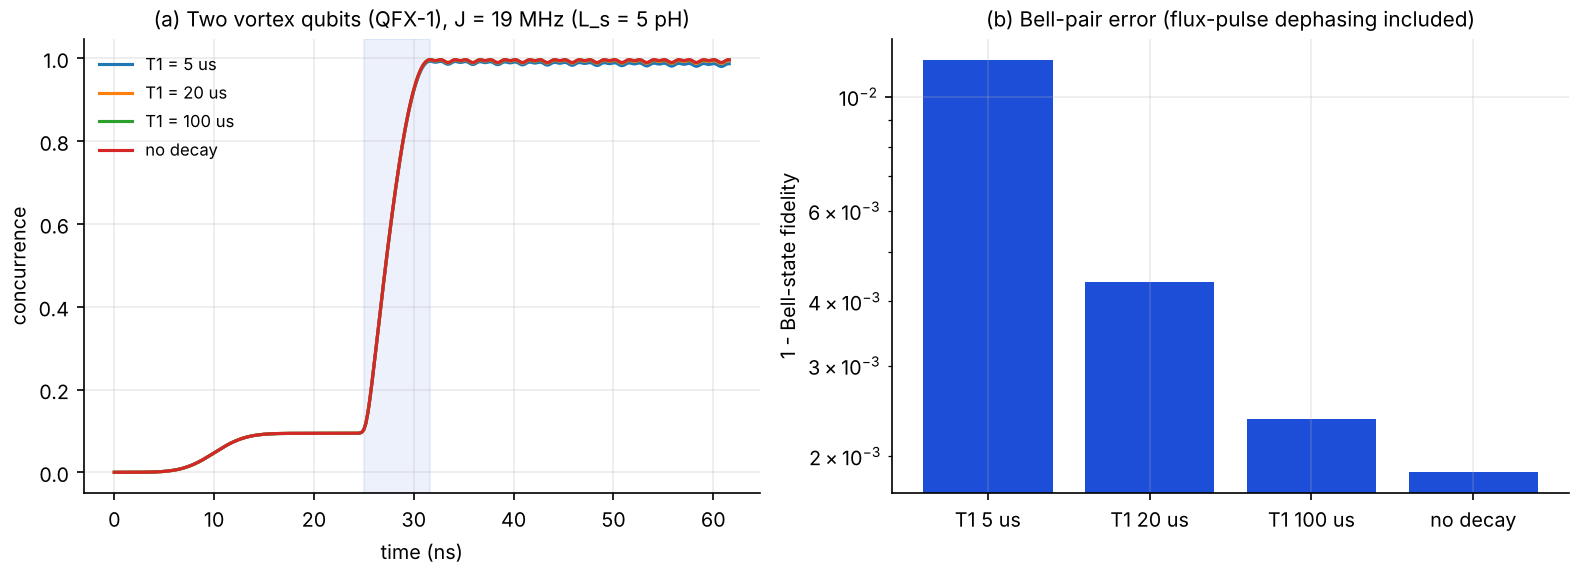
\includegraphics[width=0.62\textwidth]{../figures/companion1_bell_pair.png}\\[3pt]
{\footnotesize\textbf{(b)}}\\
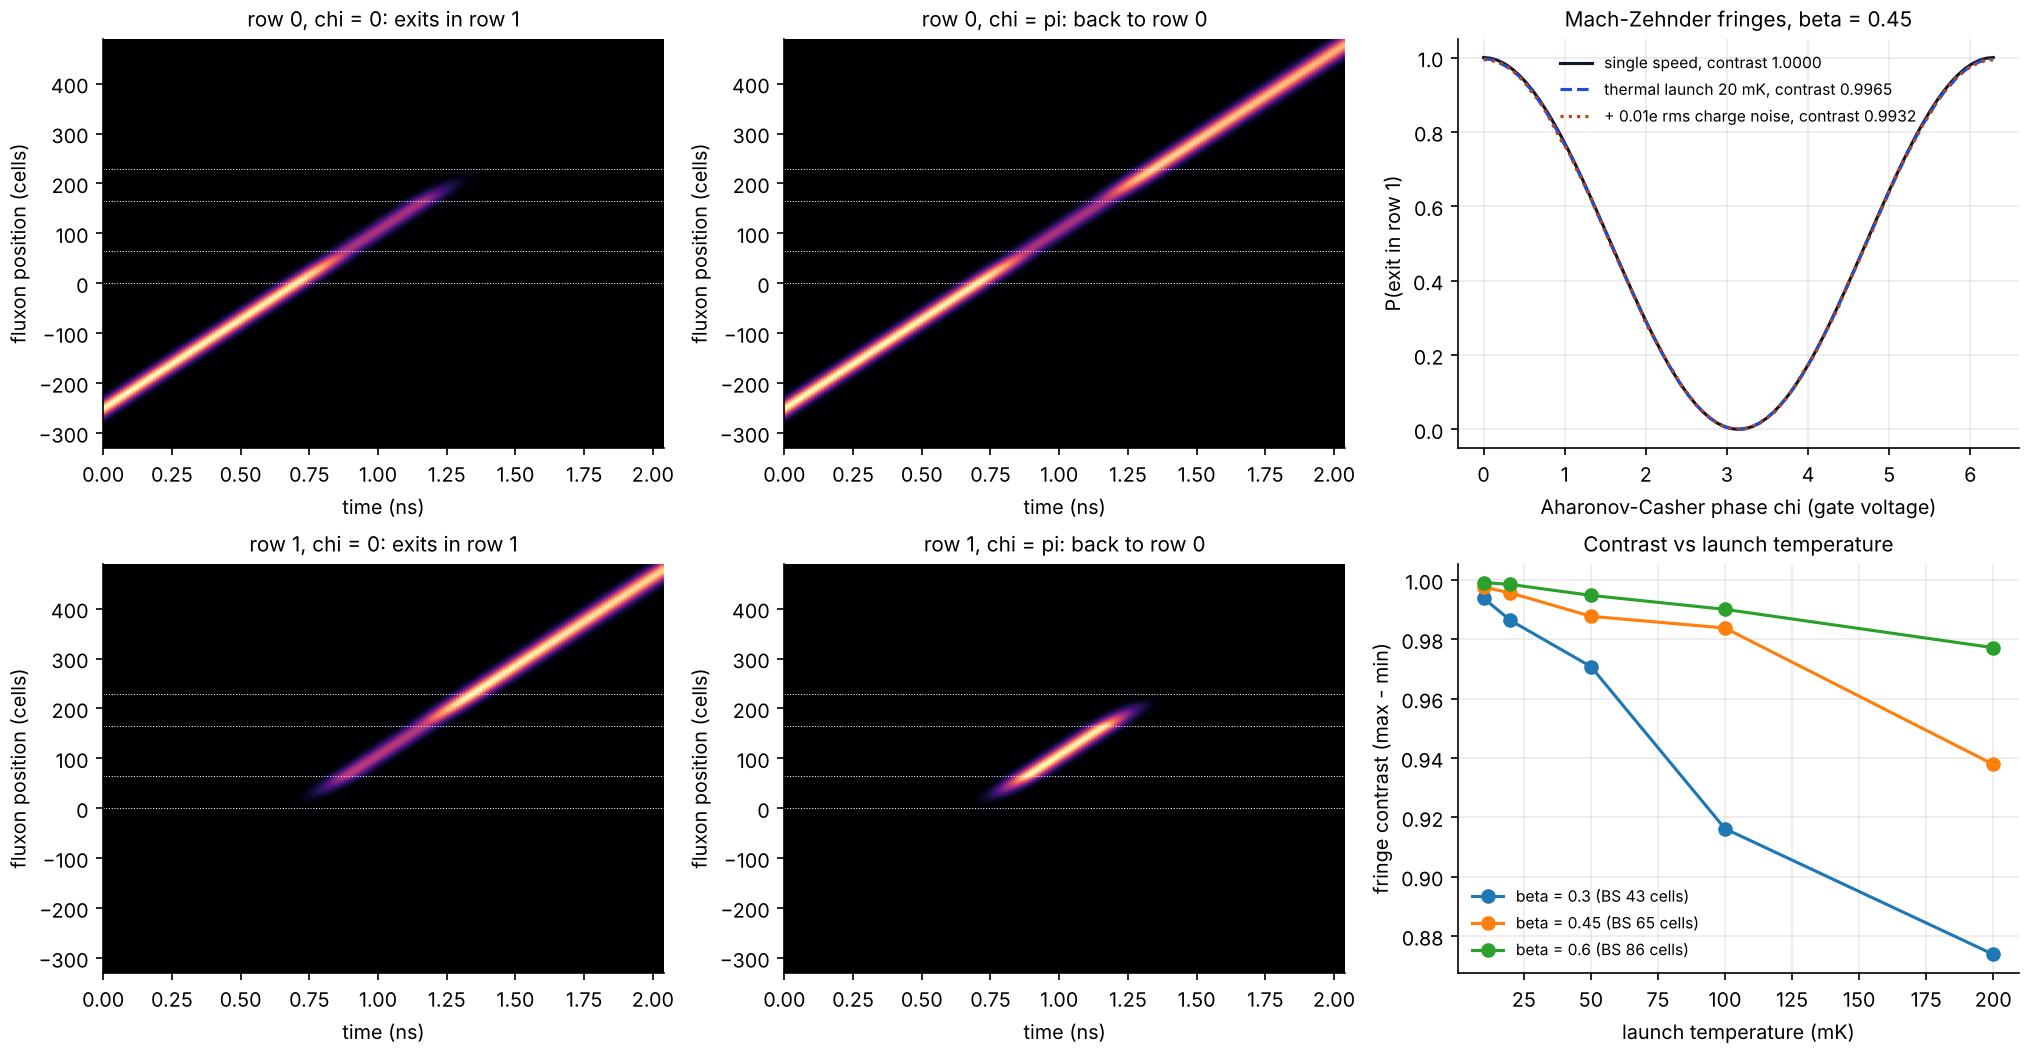
\includegraphics[width=0.74\textwidth]{../figures/companion2_router.png}\\[3pt]
{\footnotesize\textbf{(c)}}\\
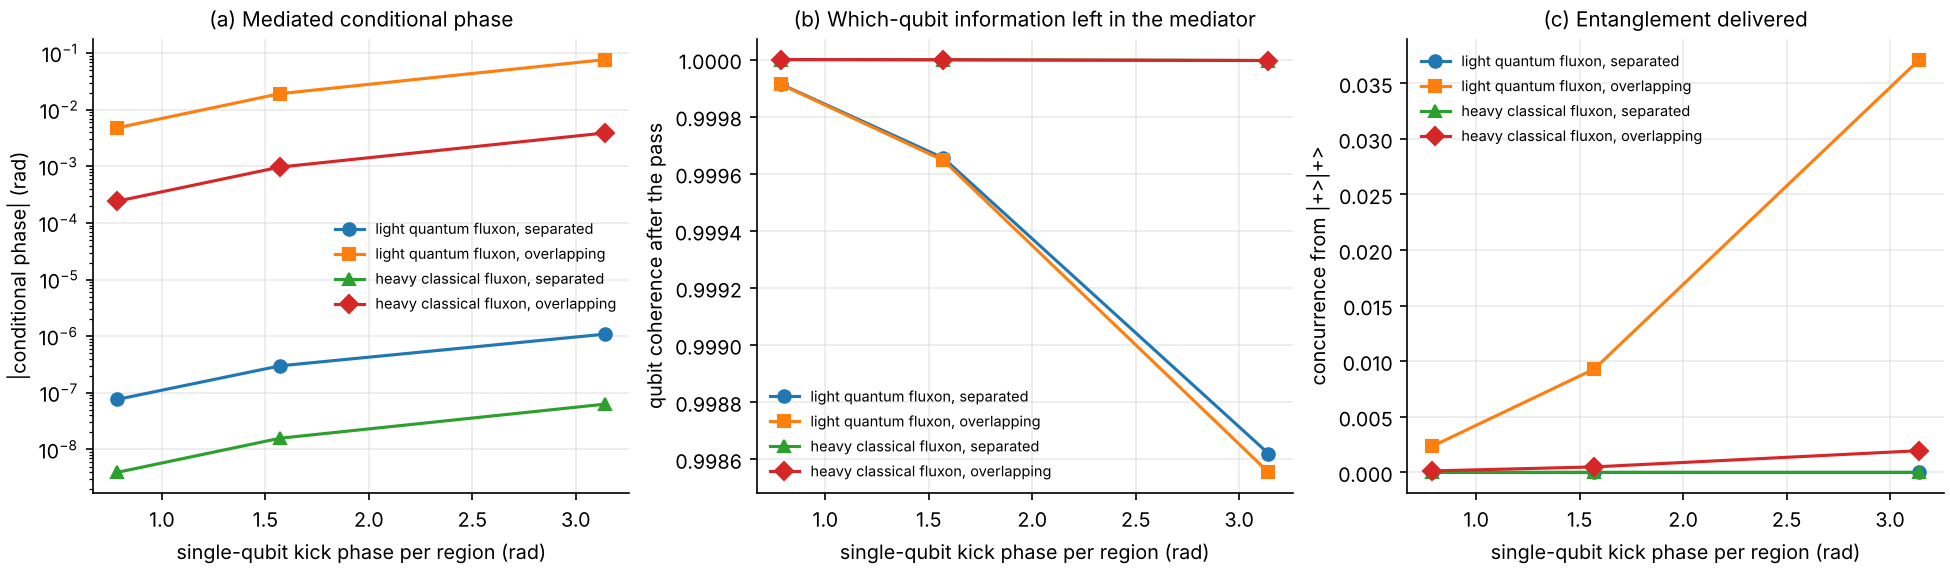
\includegraphics[width=0.74\textwidth]{../figures/companion3_mediator.png}\\[3pt]
\begin{minipage}[b]{0.53\textwidth}\centering
{\footnotesize\textbf{(d)}}\\
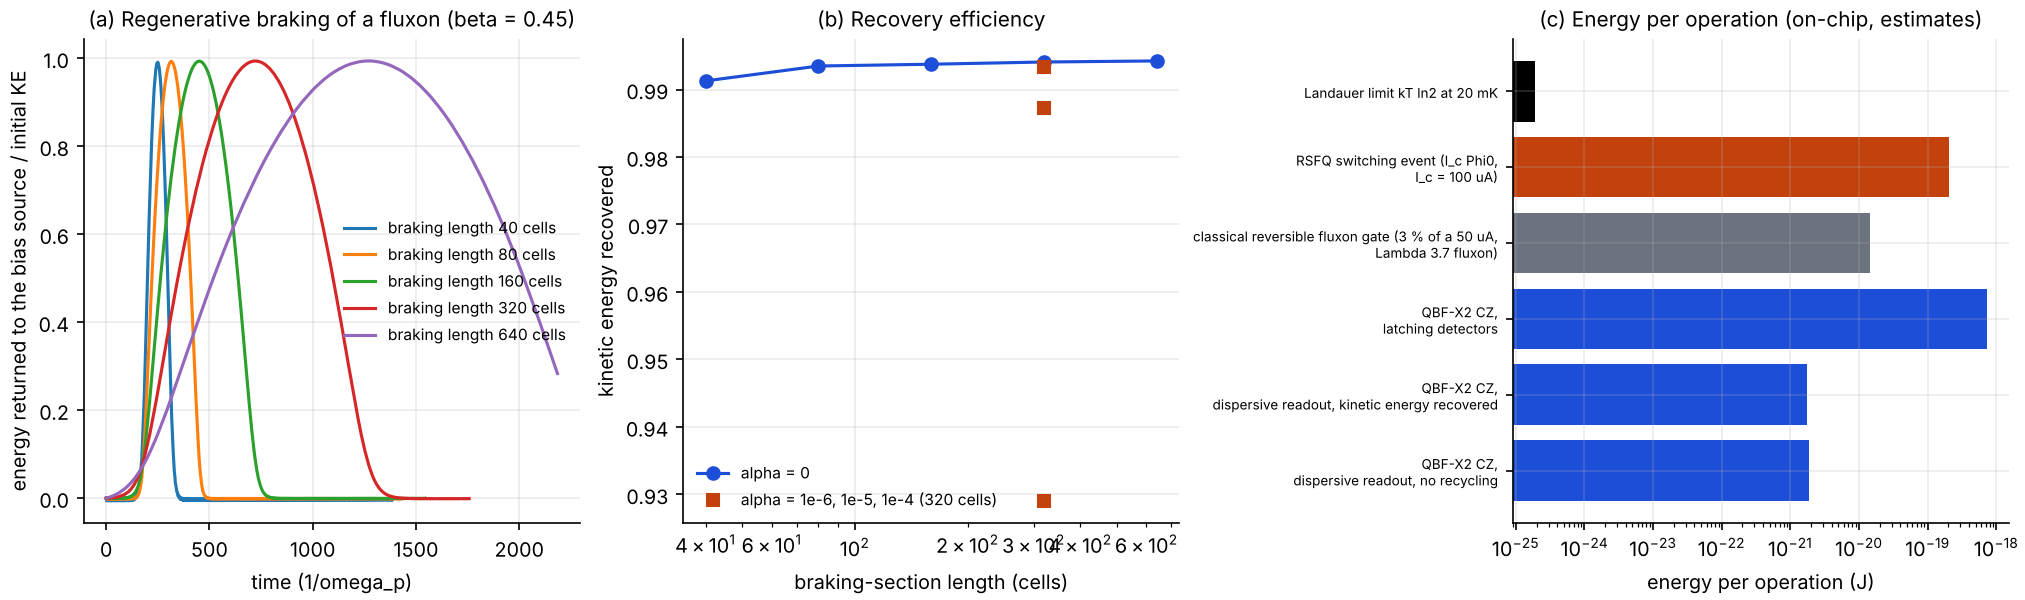
\includegraphics[width=\textwidth,trim=0 0 402.69 0,clip]{../figures/companion4_reversible_cell.png}
\end{minipage}\hspace{0.03\textwidth}%
\begin{minipage}[b]{0.37\textwidth}\centering
{\footnotesize\textbf{(e)}}\\
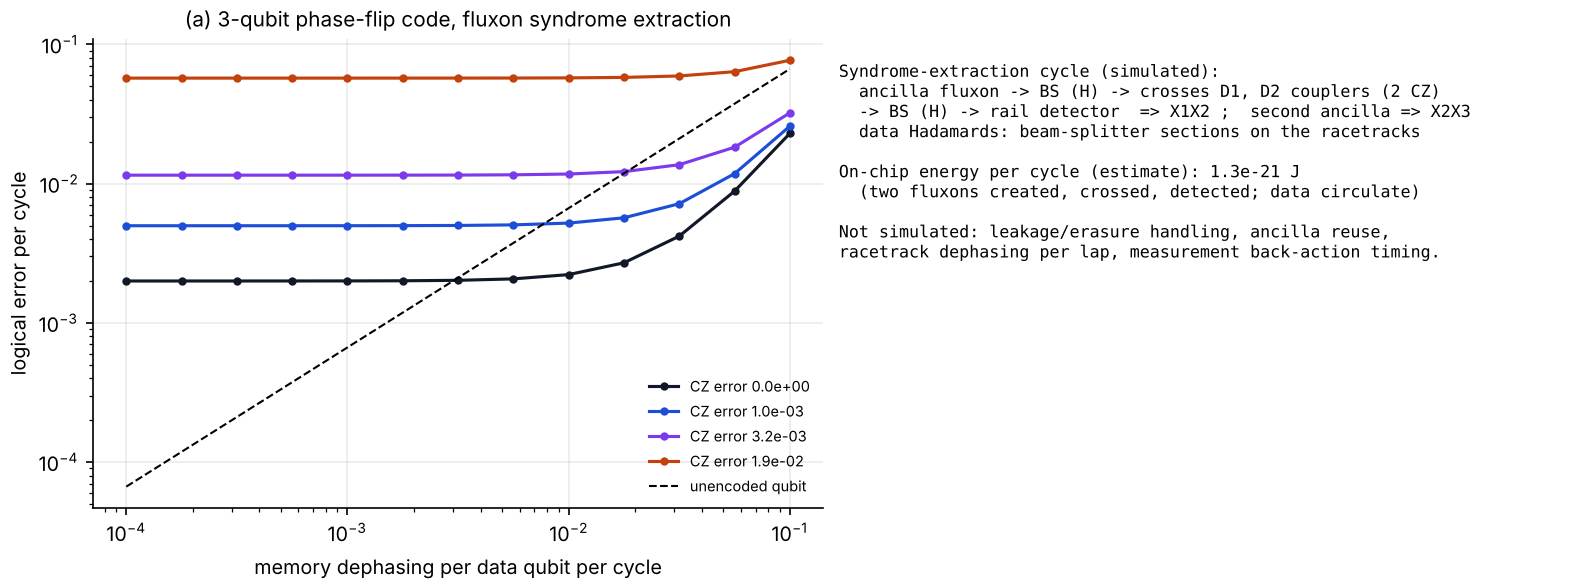
\includegraphics[width=\textwidth,trim=0 0 356.61 0,clip]{../figures/companion5_qec.png}
\end{minipage}
\caption{Companion devices (simulations only). (a)~Companion 1: concurrence during the Bell-pair protocol of two QFX-1
vortex qubits ($J=19$~MHz, $L_s=5$~pH) and Bell-state error for several $T_1$. (b)~Companion 2, fluxon router:
wavepackets entering row 0 or 1 for $\chi=0$ and $\pi$, Mach--Zehnder fringes at $\beta=0.45$ and contrast versus
launch temperature. (c)~Companion 3, negative result: mediated conditional phase, single-qubit coherence after the pass
and delivered concurrence for light and heavy mediators with separated or overlapping coupling regions.
(d)~Companion 4: regenerative braking at $\beta=0.45$ and recovery efficiency versus braking length; the
energy-per-operation panel of the source figure equals Fig.~\ref{fig:energy}(c) and is not repeated. (e)~Companion 5:
logical error per syndrome-extraction cycle versus memory dephasing for CZ errors 0, $10^{-3}$, $1.9\ee{-2}$ and
$2.0\ee{-2}$, with an unencoded qubit (dashed); the text panel of the source figure is summarised in
Sec.~\ref{sec:companions}.}
\label{fig:companions}
\end{figure*}

\section{Limitations}
\label{sec:limits}

\emph{Model.} The quantum model is a first-order theory of two collective coordinates, validated against the classical
circuit near the operating point. It breaks down below $\beta\approx0.22$ and above $\beta\approx0.35$ (inductive) to
0.45 (mixed), and the optimum lies at the edge of this range. The calibration removes the second-order phase error on
the same model, not on the full quantum circuit. Plasmon emission is estimated classically, not quantised, and the
quantum emission probability is of order $E_{\rm rad}/\hbar\omega_p$.

\emph{Not modelled.} Preparation of the launched fluxon's motional state; quasiparticles and $1/f$ noise beyond a
damping estimate; offset-charge drift of the beam-splitter islands; electromagnetic extraction of $k$, $c$ and $E_S$.
The disorder model assumes independent static cell errors, and the damping channel is an upper bound.

\emph{Design.} The layout is preliminary (no DRC, an unverified crossover process, node and island shunts not drawn
and to be set by electromagnetic extraction), and the coherent launcher, which sets the launch-speed spread on which the
whole budget depends, is unresolved.

\emph{Criteria and scope.} Three acceptance criteria were changed after results were seen (Secs.~\ref{sec:resA},
\ref{sec:resB} and~\ref{sec:device}), and the failures and the reasoning are kept in the result files. Each companion
result comes from one simulation, and companion 1 depends on the QFX-1 design and on assumed $T_1$ values. The
prior-art statements describe the sources searched. A professional patent search and a full-text review, in particular
of Ref.~\cite{Fujii2007}, are needed before any claim of invention.

\section{Conclusion}
\label{sec:conclusion}

QBF-X2 is a proposal, studied in simulation, for a CZ gate between two flying quantum fluxons. From the circuit
Lagrangian we derived a first-order collective-coordinate Hamiltonian whose interaction agrees with a constrained
relaxation of the circuit to 0.76\% at contact. Combining inductive and capacitive couplers makes the conditional phase
stationary in speed: for a design at $\beta^*=0.30$ the conditional shift crosses zero at $\beta=0.302$ in the circuit
and at 0.293 in the quantum model. With the coupler calibrated on exact 2D scattering, the gate reaches a CZ process
fidelity of 0.999999 for pure wavepackets, and its thermal error at 20~mK is $1.2\ee{-5}$ against $3.8\ee{-3}$ without
the capacitive coupler. Milestones A, B and C pass. Milestone D is not met: dephasing from junction disorder limits the
gate to a 1.9\% error at the optimised speed $\beta=0.45$, the coherent launcher is unresolved and the layout is
unverified. A sub-1\% gate requires junction disorder of 1\% or less or flights of at most 150 cells, and the proposed
experiment starts with the classical sweet-spot test.

\section*{Data and code availability}
All code, results, figures and circuit files are in the repository directory \file{qbf-x2/\allowbreak{}}. The script
\file{./\allowbreak{}run\_\allowbreak{}all.\allowbreak{}sh} reproduces every simulation, figure, circuit file and this paper (about 45~min on four CPU cores),
and \file{python -m pytest} runs 18 tests (sine-Gordon benchmarks, unitarity, eikonal limit, sweet spot, metrics,
netlist). Each stage writes \file{results/\allowbreak{}<stage>.\allowbreak{}json} with its acceptance checks; the prior-art search is documented
in \file{NOVELTY.\allowbreak{}md} and \file{results/\allowbreak{}prior\_\allowbreak{}art\_\allowbreak{}report.\allowbreak{}md}.

\appendix
\section{Milestone checks}
\label{app:milestones}

Table~\ref{tab:milestones} reproduces the milestone entries of the result files. Three criteria were changed after the
first results, and the original versions and reasons are kept in the files. (i) Milestone A first required the
first-order theory to match the circuit within 15\% over $\beta=0.25$--0.40; it failed
(\file{first\_\allowbreak{}order\_\allowbreak{}accuracy\_\allowbreak{}worst\_\allowbreak{}0.25\_\allowbreak{}0.40}${}=0.243$, i.e.\ 24\% at $\beta=0.40$) and became the accuracy map
of milestone B. (ii) Milestone B, \file{superseded\_\allowbreak{}check}: ``An earlier correspondence test compared quantum and
classical shifts only where both scans had a point with |shift| \textgreater{} 0.05 cells: one point (5.8 \%).
Replaced by the two tests above.'' (iii) Milestone D first compared the simulated outgoing kinetic energy with the
formula value $E_0(\gamma-1)$ and then used the whole-flight retention (99.877\% at $\beta=0.30$, failing
$>99.9$\%). It now applies to the gate (couplers + collision), using reference runs (Sec.~\ref{sec:device}).

\begin{table*}[t]
\centering\scriptsize
\caption{Milestone checks as stored in the result files (keys \texttt{milestone\_A}--\texttt{milestone\_D}); check names and detail strings are reproduced verbatim. A milestone passes only if every check passes.}
\label{tab:milestones}
\setlength{\tabcolsep}{4pt}\renewcommand{\arraystretch}{1.05}
\begin{tabularx}{\textwidth}{@{}>{\raggedright\arraybackslash}X c >{\raggedright\arraybackslash}p{0.40\textwidth}@{}}
\toprule
Check & Passed & Detail (verbatim)\\
\midrule
\multicolumn{3}{@{}l}{\textbf{Milestone A (classical ballistic physics): PASS}\quad(\texttt{results/A\_classical.json})}\\
energy conserved without damping & yes & max relative drift 1.2e-06\\
free fluxon speed and E = E0 gamma & yes & speed within 2 \%, energy within 1 \% for beta 0.1-0.6\\
exact sine-Gordon kink-antikink shift reproduced (Lambda = 10, beta 0.2-0.4) & yes & 0.15: 0.999, 0.2: 0.998, 0.3: 0.983, 0.4: 0.984, 0.5: 0.965\\
topological charge conserved (one fluxon per rail after the collision) & yes & windings 0.9997-1.0005 (end phases carry radiation)\\
conditional shift of the mixed coupler crosses zero at beta* = 0.30 +- 0.02 & yes & zero crossing at beta = 0.3020\\
collision-induced radiation \textless{} 1e-3 of the pair kinetic energy (mixed coupler) & yes & max 2.2e-04\\
\midrule
\multicolumn{3}{@{}l}{\textbf{Milestone B (quantum ballistic physics): PASS}\quad(\texttt{results/B\_quantum.json})}\\
unitarity: norm conserved & yes & max drift 3.0e-08\\
converged: phase within 0.01 rad under dt, dx (k cut-off), domain and Taylor-order changes & yes & phase spread 0.0007 rad over 6 runs\\
coherent single-fluxon propagation: group velocity and dispersion match the relativistic E(k) & yes & v\_g 238.22 vs 238.43 cells/ns, width 45.93 vs 45.94 cells\\
topological charge: the collision is reflectionless (both fluxons transmitted) & yes & reflection 7.1e-08\\
quantum-classical correspondence: conditional-delay zero crossing, quantum vs classical circuit, within 0.02 in beta & yes & quantum 0.2933, classical circuit 0.3020\\
quantum corrections to the classical limit of the same model \textless{} 10 \% of the delay scale (all 10 points) & yes & worst 8.9 \%\\
derived interaction: first-order potential vs constrained relaxation of the circuit within 5 \% at contact & yes & +0.76 \%\\
effective-model regime: quantum (beta\textasciicircum{}2 \textasciitilde{} 0.5 \textless{} 8 pi), PN barrier \textless{}\textless{} kinetic energy & yes & beta\textasciicircum{}2 = 0.506, PN = 2.92e-06 GHz vs KE = 38.5 GHz\\
\midrule
\multicolumn{3}{@{}l}{\textbf{Milestone C (genuine quantum gate): PASS}\quad(\texttt{results/C\_gate.json})}\\
nonlocal phase: Delta = pi +- 0.01 rad (exact 2D, calibrated) & yes & Delta = 3.1432 rad\\
entanglement from \textbar{}+\textgreater{}\textbar{}+\textgreater{}: concurrence \textgreater{} 0.99 & yes & C = 1.000000\\
Bell-state fidelity \textgreater{} 0.99 (after a local Hadamard) & yes & F\_Bell = 0.999999\\
CZ average gate fidelity \textgreater{} 0.99 (pure wavepackets) & yes & F\_avg = 0.999999\\
logical, not motional, entanglement: motional Schmidt purity \textgreater{} 0.999, logical purity \textgreater{} 0.99 & yes & motional purity 0.999999, logical purity 1.000000\\
leakage (reflection / loss of a fluxon) \textless{} 1e-4 & yes & 6.2e-08\\
control: coupler off gives no entanglement & yes & C = 2.1e-08\\
thermal launch at 20 mK, sweet spot: intrinsic gate infidelity \textless{} 1e-2 & yes & 1.2e-05 (inductive-only coupler: 3.8e-03)\\
two-velocity phase model validated against 2D (\textbar{}error\textbar{} \textless{} 0.05 rad) & yes & beta\_B 0.27: 3.143 vs 3.145, beta\_B 0.33: 3.143 vs 3.138\\
\midrule
\multicolumn{3}{@{}l}{\textbf{Milestone D (device feasibility): NOT MET}\quad(\texttt{results/D\_feasibility.json})}\\
circuit parameters inside demonstrated fabrication ranges (junction \textgreater{}= 0.01 um\textasciicircum{}2, C\_c \textgreater{}= 0.1 fF, L\_s \textgreater{}= 1 pH, granular Al \textgreater{}= 1 square) & yes & rail JJ 0.038 um\textasciicircum{}2, middle JJ 0.024 um\textasciicircum{}2, C\_c 0.21 fF, L\_s 11.6 pH, grAl 1.31 sq\\
complete netlist with no floating nodes; every logical row has an injector and a catcher & yes & 8082 elements, 2877 nodes, isolated 0\\
flight time \textless{}\textless{} coherence times reported for vortex qubits (us range) & yes & 1.01 ns per pass\\
energy: kinetic energy retained through the gate (couplers + collision) \textgreater{} 99.9 \% without damping & yes & beta 0.30: gate 0.99998 (whole flight incl. launch transient 0.99877), beta 0.45: gate 0.99997 (whole flight incl. launch transient 0.99916)\\
error budget at the optimum \textless{} 1 \% with 2 \% junction disorder, 20 mK launch, 10 ps jitter (realistic assumptions) & \textbf{no} & total 0.0191: gate\_thermal 1.3e-06, disorder\_dephasing 1.8e-02, damping 1.5e-03, timing 0.0e+00, coupler 0.0e+00\\
coherent single-fluxon launcher derived (timing \textless{}= 10 ps, thermal-limited speed spread) & \textbf{no} & UNRESOLVED: injector pulse + accelerator proposed, motional-state preparation not modelled\\
layout verified (DRC, EM extraction of k, c, E\_S) & \textbf{no} & NOT DONE: preliminary layout only\\
\bottomrule
\end{tabularx}
\end{table*}

\begin{thebibliography}{99}

\bibitem{Kurpiers2018}
P.~Kurpiers \emph{et al.}, Nature \textbf{558}, 264 (2018), \doi{10.1038/s41586-018-0195-y}.

\bibitem{Axline2018}
C.~J. Axline \emph{et al.}, Nat. Phys. \textbf{14}, 705 (2018), \doi{10.1038/s41567-018-0115-y}.

\bibitem{CampagneIbarcq2018}
P.~Campagne-Ibarcq \emph{et al.}, Phys. Rev. Lett. \textbf{120}, 200501 (2018), \doi{10.1103/PhysRevLett.120.200501}.

\bibitem{Bertoni2000}
A.~Bertoni, P.~Bordone, R.~Brunetti, C.~Jacoboni, and S.~Reggiani, Phys. Rev. Lett. \textbf{84}, 5912 (2000),
\doi{10.1103/PhysRevLett.84.5912}.

\bibitem{Ionicioiu2001}
R.~Ionicioiu, G.~A.~J. Amaratunga, and F.~Udrea, Int. J. Mod. Phys. B \textbf{15}, 125 (2001),
\doi{10.1142/S0217979201003521}.

\bibitem{Fletcher2023}
J.~D. Fletcher \emph{et al.}, Nat. Nanotechnol. (2023), \doi{10.1038/s41565-023-01369-4}.

\bibitem{Ubbelohde2023}
N.~Ubbelohde \emph{et al.}, Nat. Nanotechnol. (2023), \doi{10.1038/s41565-023-01370-x}.

\bibitem{Wang2023}
J.~Wang \emph{et al.}, Nat. Nanotechnol. (2023), \doi{10.1038/s41565-023-01368-5}.

\bibitem{Ustinov1998}
A.~V. Ustinov, ``Solitons in Josephson junctions,'' Physica D \textbf{123}, 315 (1998),
\doi{10.1016/S0167-2789(98)00131-6}.

\bibitem{WustmannOsborn2020}
W.~Wustmann and K.~D. Osborn, ``Reversible fluxon logic: Topological particles allow ballistic gates along
one-dimensional paths,'' Phys. Rev. B \textbf{101}, 014516 (2020), \doi{10.1103/PhysRevB.101.014516},
\arxiv{1711.04339}.

\bibitem{Osborn2017}
K.~D. Osborn, ``Reversible computation with flux solitons,'' US Patent 9,812,836 (filed 2014, granted 2017); claims
not read.

\bibitem{Wallraff2003}
A.~Wallraff \emph{et al.}, Nature \textbf{425}, 155 (2003), \doi{10.1038/nature01826}.

\bibitem{SeidovFistul2021}
S.~S. Seidov and M.~V. Fistul, Phys. Rev. A \textbf{103}, 062410 (2021), \doi{10.1103/PhysRevA.103.062410}.

\bibitem{Wildermuth2023}
M.~M. Wildermuth, ``Quantum Tunneling of Josephson Vortices in High-Impedance Long Junctions,'' dissertation, KIT
(2023), \doi{10.5445/IR/1000158804}.

\bibitem{Nambisan2026}
A.~Nambisan, S.~G{\"u}nzler, D.~Rieger, \ldots, M.~Spiecker, and I.~M. Pop, ``Quantum coherent manipulation and
readout of superconducting vortex states,'' Nature \textbf{653}, 63--67 (2026), \doi{10.1038/s41586-026-10441-7},
\arxiv{2510.19769}.

\bibitem{RelatedPatents}
Related classical patents (titles from search listings, claims not read): US 10,778,229 B1 (Osborn, Wustmann);
US 11,289,156 B2 and US 12,620,993 B1 (Sandia); US 12,166,259 B1 (NSA).

\bibitem{WustmannOsborn2026}
W.~Wustmann and K.~D. Osborn, ``Rapid qubit readout dependent on the transmission of a single fluxon,'' Phys. Rev.
Applied \textbf{25} (2026), \doi{10.1103/lq5c-3j66}; preprint \arxiv{2504.18915}. The article number 034027 quoted
for this paper could not be verified.

\bibitem{Sakai1993}
S.~Sakai, P.~Bodin, and N.~F. Pedersen, J. Appl. Phys. \textbf{73}, 2411 (1993), \doi{10.1063/1.353095}.

\bibitem{Kleiner1994}
R.~Kleiner, Phys. Rev. B \textbf{50}, 6919 (1994), \doi{10.1103/PhysRevB.50.6919}.

\bibitem{KivsharMalomed1988}
Y.~S. Kivshar and B.~A. Malomed, Phys. Rev. B \textbf{37}, 9325 (1988), \doi{10.1103/PhysRevB.37.9325}.

\bibitem{GronbechJensen1994}
N.~Gr{\o}nbech-Jensen \emph{et al.}, Phys. Rev. B \textbf{50}, 6352 (1994), \doi{10.1103/PhysRevB.50.6352}.

\bibitem{UstinovKohlstedt1996}
A.~V. Ustinov and H.~Kohlstedt, Phys. Rev. B \textbf{54}, 6111 (1996), \doi{10.1103/PhysRevB.54.6111}.

\bibitem{Fujimaki1987}
A.~Fujimaki \emph{et al.}, Phys. Rev. Lett. \textbf{59}, 2895 (1987), \doi{10.1103/PhysRevLett.59.2895}.

\bibitem{Nakajima1990}
K.~Nakajima \emph{et al.}, Phys. Rev. Lett. \textbf{65}, 1667 (1990), \doi{10.1103/PhysRevLett.65.1667}.

\bibitem{Zamolodchikov1979}
A.~B. Zamolodchikov and Al.~B. Zamolodchikov, Ann. Phys. \textbf{120}, 253 (1979),
\doi{10.1016/0003-4916(79)90391-9}.

\bibitem{RoySaleur2019}
A.~Roy and H.~Saleur, ``Quantum electronic circuit simulation of generalized sine-Gordon models,'' Phys. Rev. B
\textbf{100}, 155425 (2019), \doi{10.1103/PhysRevB.100.155425}.

\bibitem{Roy2021}
A.~Roy, D.~Schuricht, J.~Hauschild, F.~Pollmann, and H.~Saleur, ``The quantum sine-Gordon model with quantum
circuits,'' Nucl. Phys. B \textbf{968}, 115445 (2021), \doi{10.1016/j.nuclphysb.2021.115445}.

\bibitem{Rosen2026}
I.~T. Rosen \emph{et al.}, \arxiv{2610.11071} (2026).

\bibitem{Wildermuth2022}
M.~M. Wildermuth \emph{et al.}, Appl. Phys. Lett. \textbf{120}, 112601 (2022), \doi{10.1063/5.0082197}.

\bibitem{Elion1993}
W.~J. Elion, J.~J. Wachters, L.~L. Sohn, and J.~E. Mooij, Phys. Rev. Lett. \textbf{71}, 2311 (1993),
\doi{10.1103/PhysRevLett.71.2311}.

\bibitem{vanOudenaarden1996}
A.~van Oudenaarden and J.~E. Mooij, Phys. Rev. Lett. \textbf{76}, 4947 (1996), \doi{10.1103/PhysRevLett.76.4947}.

\bibitem{Pop2012}
Pop \emph{et al.}, Phys. Rev. B \textbf{85}, 094503 (2012).

\bibitem{Moskalenko2021}
I.~N. Moskalenko \emph{et al.}, Phys. Rev. B \textbf{103}, 224528 (2021).

\bibitem{vanderZant1992}
H.~S.~J. van der Zant, F.~C. Fritschy, T.~P. Orlando, and J.~E. Mooij, ``Ballistic vortices in Josephson-junction
arrays,'' Europhys. Lett. \textbf{18}, 343 (1992), \doi{10.1209/0295-5075/18/4/011}.

\bibitem{Fujii2007}
T.~Fujii, T.~Shibata, M.~Nishida, and N.~Hatakenaka, ``Flying superconducting qubits,'' IEEE Trans. Appl. Supercond.
\textbf{17}, 97 (2007), \doi{10.1109/TASC.2007.898035}; only the abstract was read.

\bibitem{Fujii2008}
T.~Fujii, M.~Nishida, and N.~Hatakenaka, Phys. Rev. B \textbf{77}, 024505 (2008), \doi{10.1103/PhysRevB.77.024505}.

\bibitem{Matsuo2007}
S.~Matsuo, K.~Furuta, T.~Fujii, K.~Nagai, and N.~Hatakenaka, Appl. Phys. Lett. \textbf{91}, 093103 (2007),
\doi{10.1063/1.2772770}.

\bibitem{Fujii2009}
T.~Fujii, S.~Matsuo, and N.~Hatakenaka, ``Quantum knitting computer,'' \arxiv{0905.2246} (2009).

\bibitem{Fujii2016}
T.~Fujii, S.~Matsuo, and N.~Hatakenaka, ``Fluxon-controlled quantum computer,'' Int. J. Quantum Inf. \textbf{14},
1650040 (2016), \doi{10.1142/S0219749916500404}.

\bibitem{DengAverin2014}
Q.~Deng and D.~V. Averin, ``nSQUID arrays as conveyers of quantum information,'' JETP (2014) 1152--1162,
\doi{10.1134/S1063776114120012}.

\bibitem{FistulUstinov2003}
M.~V. Fistul and A.~V. Ustinov, Phys. Rev. B \textbf{68}, 132509 (2003), \doi{10.1103/PhysRevB.68.132509}.

\bibitem{DWavePatent}
Ustinov, Walraff [sic], and Koval, US Patent 6,627,915 B1 (D-Wave, 2003); claims not read.

\bibitem{BoseKorepin2011}
S.~Bose and V.~Korepin, \arxiv{1106.2329} (2011).

\bibitem{Banchi2017}
L.~Banchi \emph{et al.}, Quantum \textbf{1}, 36 (2017), \doi{10.22331/q-2017-11-30-36}.

\bibitem{BrodCombes2016}
D.~J. Brod and J.~Combes, Phys. Rev. Lett. \textbf{117}, 080502 (2016), \doi{10.1103/PhysRevLett.117.080502}.

\end{thebibliography}

\end{document}
